\documentclass[preprint,
amsmath,amssymb,
aip,
jap,
floatfix,]{revtex4-2}

\usepackage{graphicx}
\usepackage{dcolumn}
\usepackage{bm}
\usepackage{siunitx}
\usepackage{xcolor, soul}
\usepackage{calc}
 % \usepackage{titling}
 \definecolor{Red}{RGB}{163, 25, 25}
 \usepackage{enumitem}
 \usepackage{titlesec}
   \titleformat{\chapter}[display]
  	{\normalfont\huge\bfseries}
  	{\filcenter\underline}
  	{\filcenter\underline{\MakeUppercase{\textls[400]{\chaptertitlename}}\ \thechapter}}{20pt}{\Huge}


 \titleformat{\section}
	{\bfseries\color{Red} \Large}
 	{}
 	{0em}
 	{}[\titlerule]

	
 \titleformat{\subsection}
 {\bfseries\color{Red}}
 {}
 {0em}
 {}


 \titleformat{\subsubsection}[runin]
 {\bfseries}
 {}
 {0em}
 {}
\titlespacing{\subsubsection}
{0pt}
{0.01in}
{0.08in}
{}

\titlespacing{\subsection}
{0pt}
{0.05in}
{0.05in}
\titlespacing{\section}
{0pt}
{0.05in}
{0.05in}

 \titleformat{\subsubsubsection} 
 {\bfseries}
 {}
 {0.1in}
 {}


\begin{document}




	\title{An investigation of the coupling of phonon-polaritons with
	plasmon-polaritons in a layered structure comprising of hBN on a nanopatterned square array of cross apertures in Au}

	\maketitle
	\section{Introduction}
	\label{sec:Intro}
		Optical metamaterials are artificially engineered periodic structures designed to exhibit optical properties not otherwise found in nature. Metamaterials have been used to relize applications such as negative refraction\cite{Shelby:01} and ultrahigh absorption\cite{Yang:21}. Plasmonic metamaterials  which support localized surface plasmon resonances can confine electromagnetic fields at a subwavelength scale, thereby enhancing the near-field coupling effects and light-matter interactions\cite{Cheng:15}. By varying geometrical parameters metamaterial devices have been shown to have highly tunable plasmonic resonances\cite{LiuNL:10}. Coupling between plasmonic resonances and material phonon resonances through near-field interactions can give rise to a splitting of plasmon-phonon modes with anti-crossing behaviour\cite{Shelton:11, Zhang:07}. Strong coupling can be controlled using the capacitence of metamaterial nanocavities\cite{Benz:15}.

		Several studies have been performed on hBN-metamaterial devices. These include arrays of hBN nanoparticles\cite{Caldwell:14}, an hBN sheet over a triangular lattice of circular apertures in $\mathrm{SiO}_{2}$\cite{Yang:20}, and hBN/metal-grating anisotropic structures\cite{Zhao:17}. The device studied in this chapter is an infinite hBN sheet over a square array of cross shaped apertures in Au. The cross shape offers the advantage of 4 geometric parameters that may be varied to tune the grating's plasmonic resonance to the TO resonance of hBN. These parameters are the Au film thickness ($d_\mathrm{hBN}$), cross length ($l$), cross width ($w$), and periodicity ($d_\mathrm{CC}$), which must be congruent in the $x$- and $y$- directions to maintain a square array structure. Cross-shaped apertures in Au have been shown to exhibit perfect infrared absorption\cite{Cheng:14} as well as promoting strong plasmon-phonon coupling in an IR resonant material between the grating and the source\cite{Wan:16}. $\mathrm{SiO}_{2}$was chosen as a substrate as it can be approximated as optically inert at IR frequencies.     

		\section{Preliminary Measurements}
		\label{sec:Prelim}
		The system modelled in this chapter was an hBN film atop of nanopatterned (a square array of crosses) etched into a gold (Au) film which was deposited on a fused silica ($\mathrm{SiO_2}$) substrate. The combination of the nanopatterned crosses in an Au film was selected as the plasmonic metamaterial layer because the absorption features associated with this device exhibited simpler lineshapes than those calculated for similar devices, \textit{e.g.}, circular holes in either an Ag or Au metal film.

		Data in this chaper were produced by computer simulations using the FDTD method as detailed in \textcolor{cyan}{Chapter 2 [ref]}. Due to the large time constants of the hBN and Au films incorporated in the devices studied in this investigation, $\geq 2 \times 10^6$ time steps were needed for each simulation. This necessitated incorporating GPU acceleration into the in-house code to reduce the runtime required. A combination of OpenACC and CUDA \cite{PGI:20} methodologies were used to speed up simulations by a factor of $\sim 70$; this enabled a greater number of higher resolution simulations to be performed in a reasonable time frame.

		The details of the principle nanopatterned structure simulated in this chapter are shown in Fig.~\ref{fig:3.1}. The structure was composed of an $80\, \si{\nm}$ sheet of hexagonal boron nitride (hBN) deposited on a $50\, \si{\nm}$ thick film of nanopatterned Au atop of a $\mathrm{SiO}_{2}$ substrate. The Au film was patterned with cross-shaped apertures. The aperture dimensions were $l = 0.8 \, d_\mathrm{CC}$ and $w = 0.15 \, d_\mathrm{CC}$, where $d_\mathrm{CC}$ was the model periodicity in the congruent $x$- and $y$- dimensions, which was varied during this work. 

		For all simulations performed a broadband, plane wave source was used. The time profile of the source was a Ricker wavelet \cite{Ricker:43} centered on $\lambda = 2.4\, \si{\um}$ ($4167\, \mathrm{cm}^{-1}$). This source injected a laterally uniform in time pulse using the total-field scattered-field (TFSF) interface \cite{Merewether:80}. The source was $y$-polarized and propagated in the negative $z$-direction. The use of the TFSF method enabled sensors to be placed above the TFSF boundary in order to record only the reflected field values.
		
		To prevent divergence in the simulation caused by edge reflections in the patterned Au layer, a convolutional perfectly matched layer (CPML) \cite{Gvozdic:17} boundary was used as the CPML has been shown to be more stable than a uniaxial perfectly matching layer (UPML) \cite{Sacks:95} absorbing boundary for simulations of this kind. Periodic boundary conditions were used in the transverse directions. In the positive and negative $z$-directions, the simulation was terminated by 50 perfectly matched layers. Due to the difference between the length scales of features in the transverse and longitudinal directions, the computational grid used cell sizes in the ratio of 10:10:1 in the $x$-, $y$- and $z$-dimensions, respectively. The resonance frequency of the patterned Au layer was found to be sensitive to the spatial resolution used in the simulation. Convergence testing was performed and a working resolution of $\mathrm{\Delta}x = 20 \, \si{\nm}, \ \mathrm{\Delta}y = 20 \, \si{\nm}, \ \mathrm{\Delta}z = 2 \, \si{\nm}$ was selected to be a good compromise between simulation accuracy and GPU memory limits.

		As discussed in detail in \textcolor{cyan}{Chapter 2 [ref]} the various components of the device were modelled as follows. The hBN layer was simulated using a tensor Lorentz model. The Au film was simulated using wavelength dependent refractive index data as detailed by Ciesielski \textit{et al.}  \cite{Ciesielski:18} to fit to a Debye/Drude model. Finally, the $\mathrm{SiO}_{2}$ substrate was simulated using a simple dielectric with $\varepsilon_\mathrm{SiO_2} = 2.127$. In order to validate the models of the dispersive materials used in this work, thin films of Au and hBN in vacuo were simulated and the normal incidence absorptance, $A(\omega)$, spectrum for each of the films was calculated using $A(\omega) = 1 - [T(\omega) + R(\omega)]$, where $T(\omega)$ and $R(\omega)$ are the transmittance and reflectance spectra, respectively. These absorptance spectra were compared with the absorptance spectra calculated for the corresponding film using the transfer matrix (TM) method \cite{MacLeod:01} and excellent agreement between the two methods was observed.

		In addition to the structure, denoted the ``coupled device" (CD), depicted in Fig.~\ref{fig:3.1}, several other auxiliary structures were simulated. The ``bare device" (BD), this device is identical to the coupled device, but  with the hBN layer removed. This device does not support phonon-polaritons. The  ``uncoupled device I" (UDCI), this device is identical to the coupled device, but  with the hBN layer replaced with an equal thickness anisotropic layer that has $\varepsilon_{k}(\infty)$ equal to the values for hBN, but the resonant behavior removed by setting $S_{k} = 0$. This device does not support phonon-polaritons. The ``uncoupled device II" (UCDII), this device is identical to the coupled device, but with the nanopatterned Au layer replaced with an equal thickness layer of nanopatterned Si modelled by a frequency independent dielectric constant, $\varepsilon_\mathrm{Si} = 11.73$; this device does not support plasmons.
		
		\begin{figure*}[!htb]
		  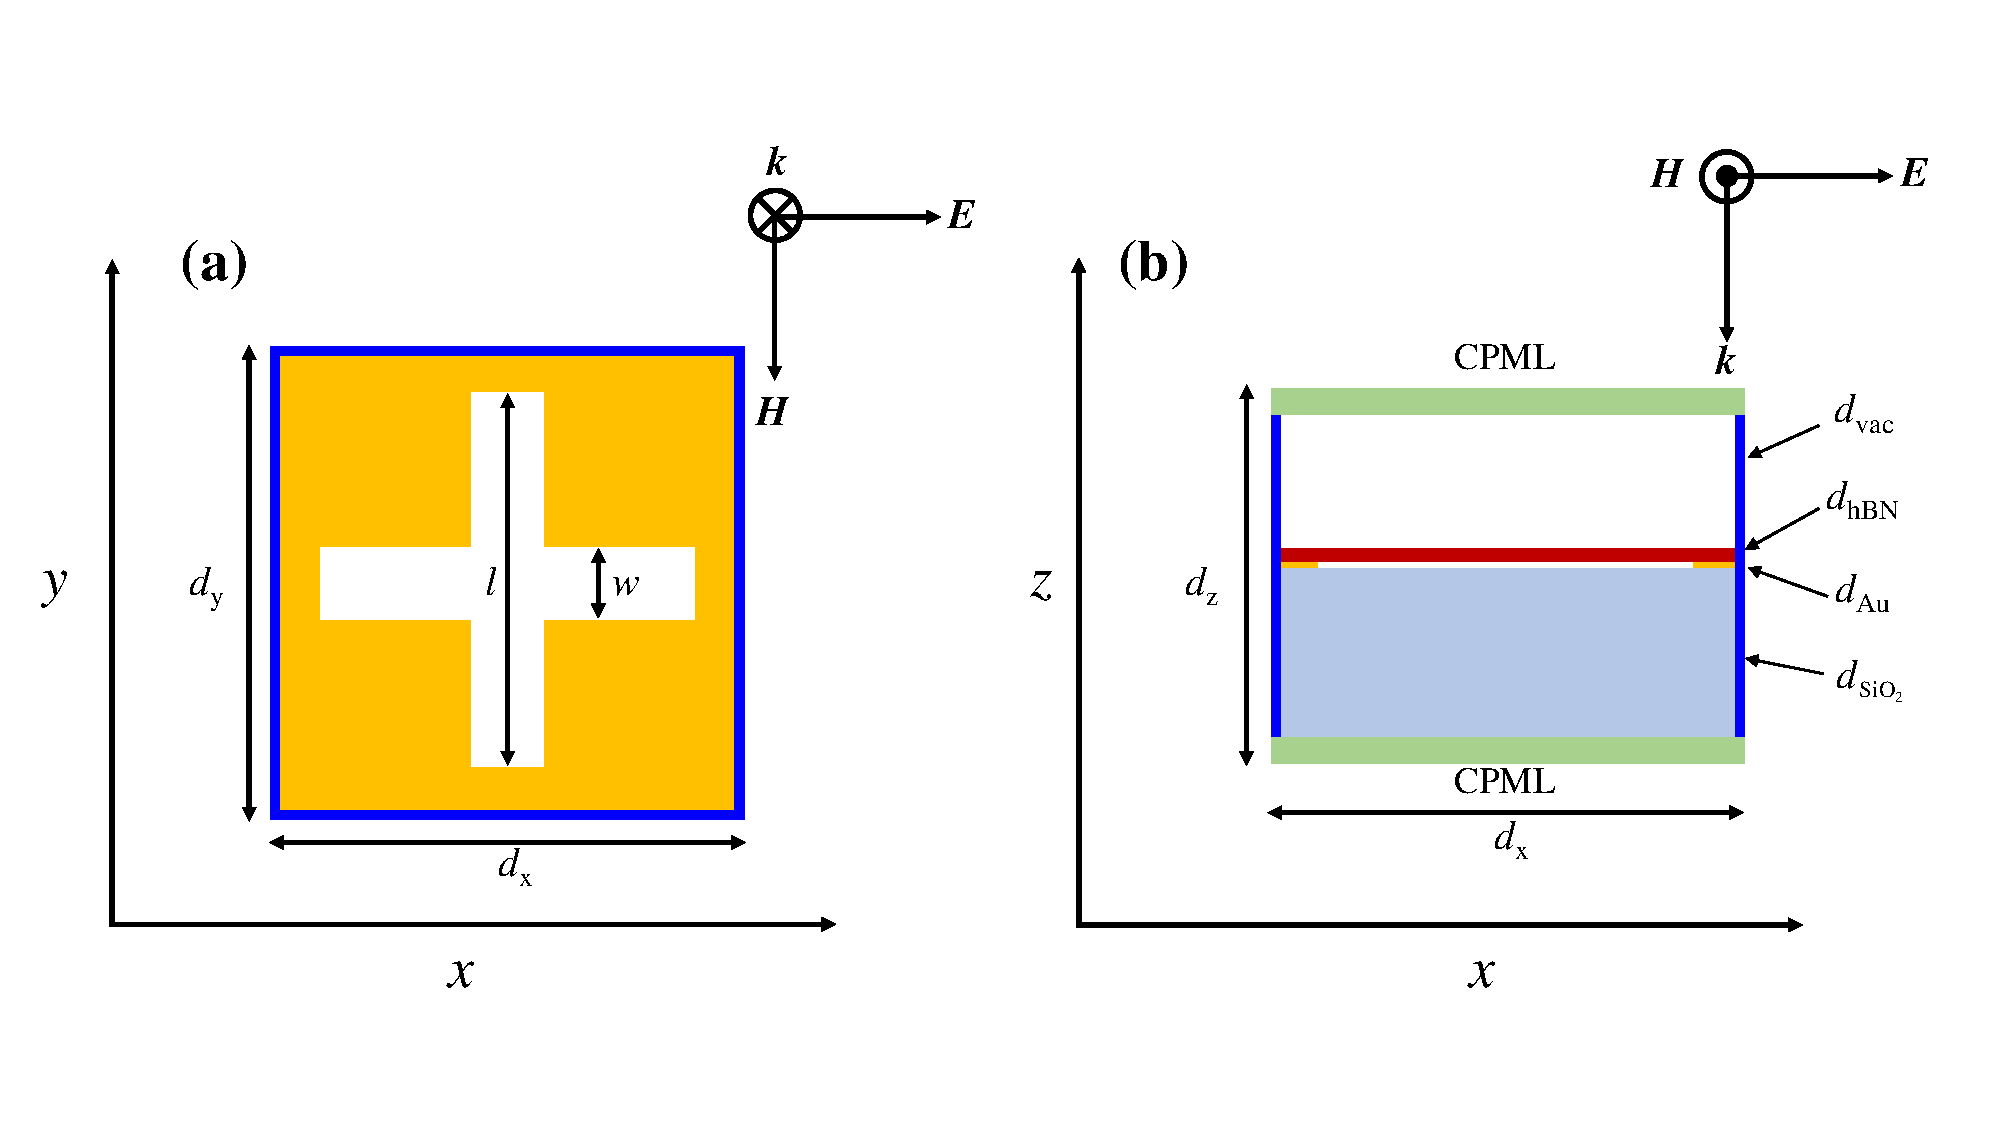
\includegraphics[width=0.9\textwidth]{Figures/Fig1.pdf}
		  \caption{Schematic of the hBN/Au structure simulated in this work. (a) Planar view at the hBN/Au interface. (b) Cross-sectional view. CPML: Convolutional perfectly matched layer boundary conditions are imposed at the $z$- direction boundaries. Periodic boundary conditions are imposed at the $x$ and $y$ boundaries. The unit cell lengths in the $x$- and $y$- directions are $d_{x} $ and $d_{y}$, respectively. The layer thicknesses are $d_\mathrm{VAC} = 0.87\, \si{\um}$, $d_\mathrm{hBN} = 80\, \si{\nm}$, $d_\mathrm{SiO_{2}} = 1.0\, \si{\um}$, $d_\mathrm{Au} = 50\, \si{\nm}$. The length of the long segments of the cross pattern is $l = 0.8 \, d_{x} = 0.8 \, d_{y}$ while the width of the cross is  $w = 0.15 \, d_{x} = 0.15 \, d_{y}$. The distance between the centers of neighboring crosses is $d_\mathrm{CC} = d_{x} = d_{y}$. The directions of the $\bm{E}$-field, $\bm{H}$-Field and propagation vector $\bm{k}$ are shown in both panes.}
		  \label{fig:3.1}
		\end{figure*}
 

		\subsection{Bare Device}
		\label{sec:BD}

		In order to investigate the effect of tuning the plasmon resonance through the hBN restrahlen band, a series of FDTD simulations were performed at a range of distances between the nearest neighbor centers of the crosses, (\textit{i.e.,} $d_\mathrm{CC}$ in the range 2.34 -- 3.94 $\si{\um}$). The resulting $R(\omega)$, $R(\omega)$, and $A(\omega)$ spectra are shown in Fig.~\ref{fig:3.2}. Two clear features can be observed in each spectra, in Fig.~\ref{fig:3.2} (c) these can be described as a smooth peak towards the red and "sShark fin" shaped peaks towards the blue end of the spectrum. The smooth peak is the plasmon resonance while the shark fin peaks are due to Rayleigh anomalies.  A clear red shift in all spectra was observed as the value of $d_\mathrm{CC}$ was increased. This demonstrated the tunability of the BD plasmon resonance. The shifted resonance of all three spectra appear to be equal in all cases. 

			\begin{figure}[!htb]
			  \centering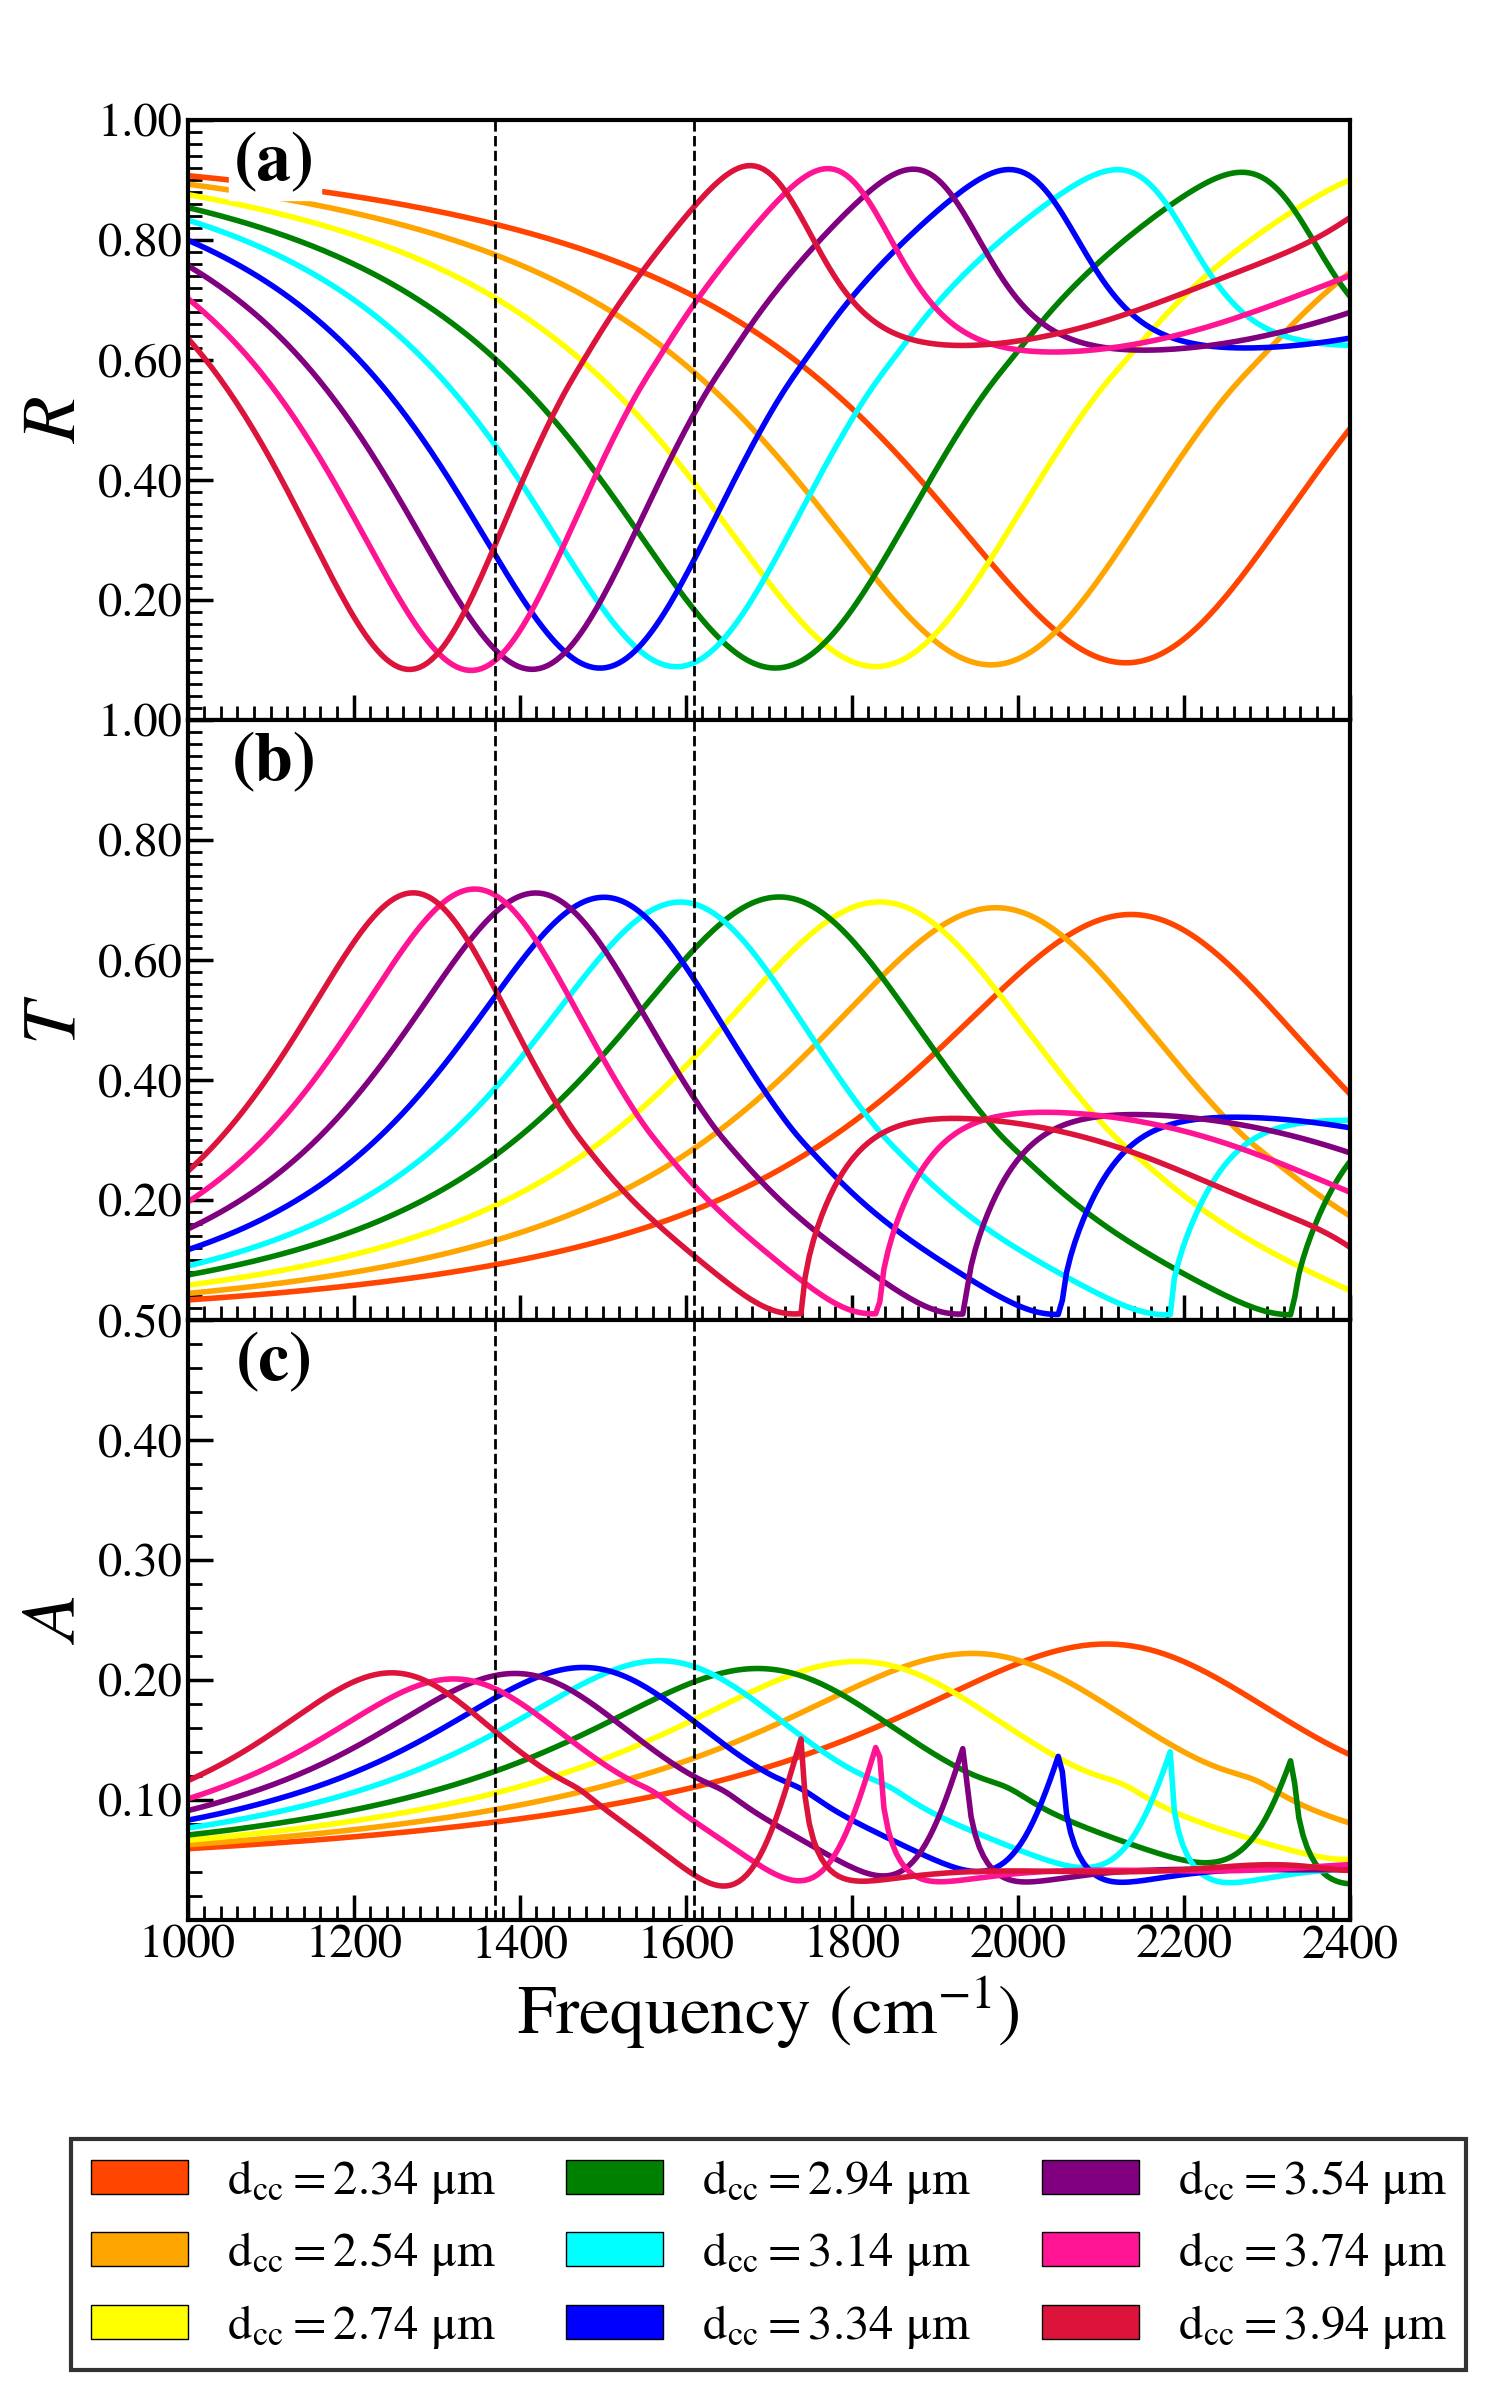
\includegraphics[width=0.45\textwidth]{Figures/BareRTA1000_2400.png}
			  \caption{The spectra for the BD at a range of $d_\mathrm{CC}$ values. (a) Reflectance spectra. (b) Transmittance spectra. (c) Absorptance spectra.  The vertical black dashed lines in this figure indicate the position of the hBN TO and LO phonon frequencies as described in \textcolor{cyan}{Chapter 2 [ref]}.}
			  \label{fig:3.2}
			\end{figure}

		\subsection{Uncoupled Device I}
		\label{sec:UCDI}
			A similar series of simulations were performed for the UCDI and are shown in Fig.~\ref{fig:3.3}. As in the BD a red shift in all spectra was oberved as the value of $d_\mathrm{CC}$ was increased. As can be seen by comparing the absorptance spectra in Fig.~\ref{fig:3.2} (c) and Fig.~\ref{fig:3.3} (c) the plasmonic resonance for each UCDI were red shifted when compared to the equivalent $d_\mathrm{CC}$ BD. However the peak frequencies of the Rayleigh anomalies remained unchanged under the same comparison. The absorptance at the plasmon resonance is increased for the UCDI while the Rayleigh anomaly magnitudes are reduced. The structure with $d_\mathrm{CC} = 3.14\,\si{\um}$ exhibits a plasmon absorptance peak that is most closely resonant with the hBN TO phonon and this device is the one studied most extensively in the near field analasis section of this chapter.

			\begin{figure}[!htb]
			  \centering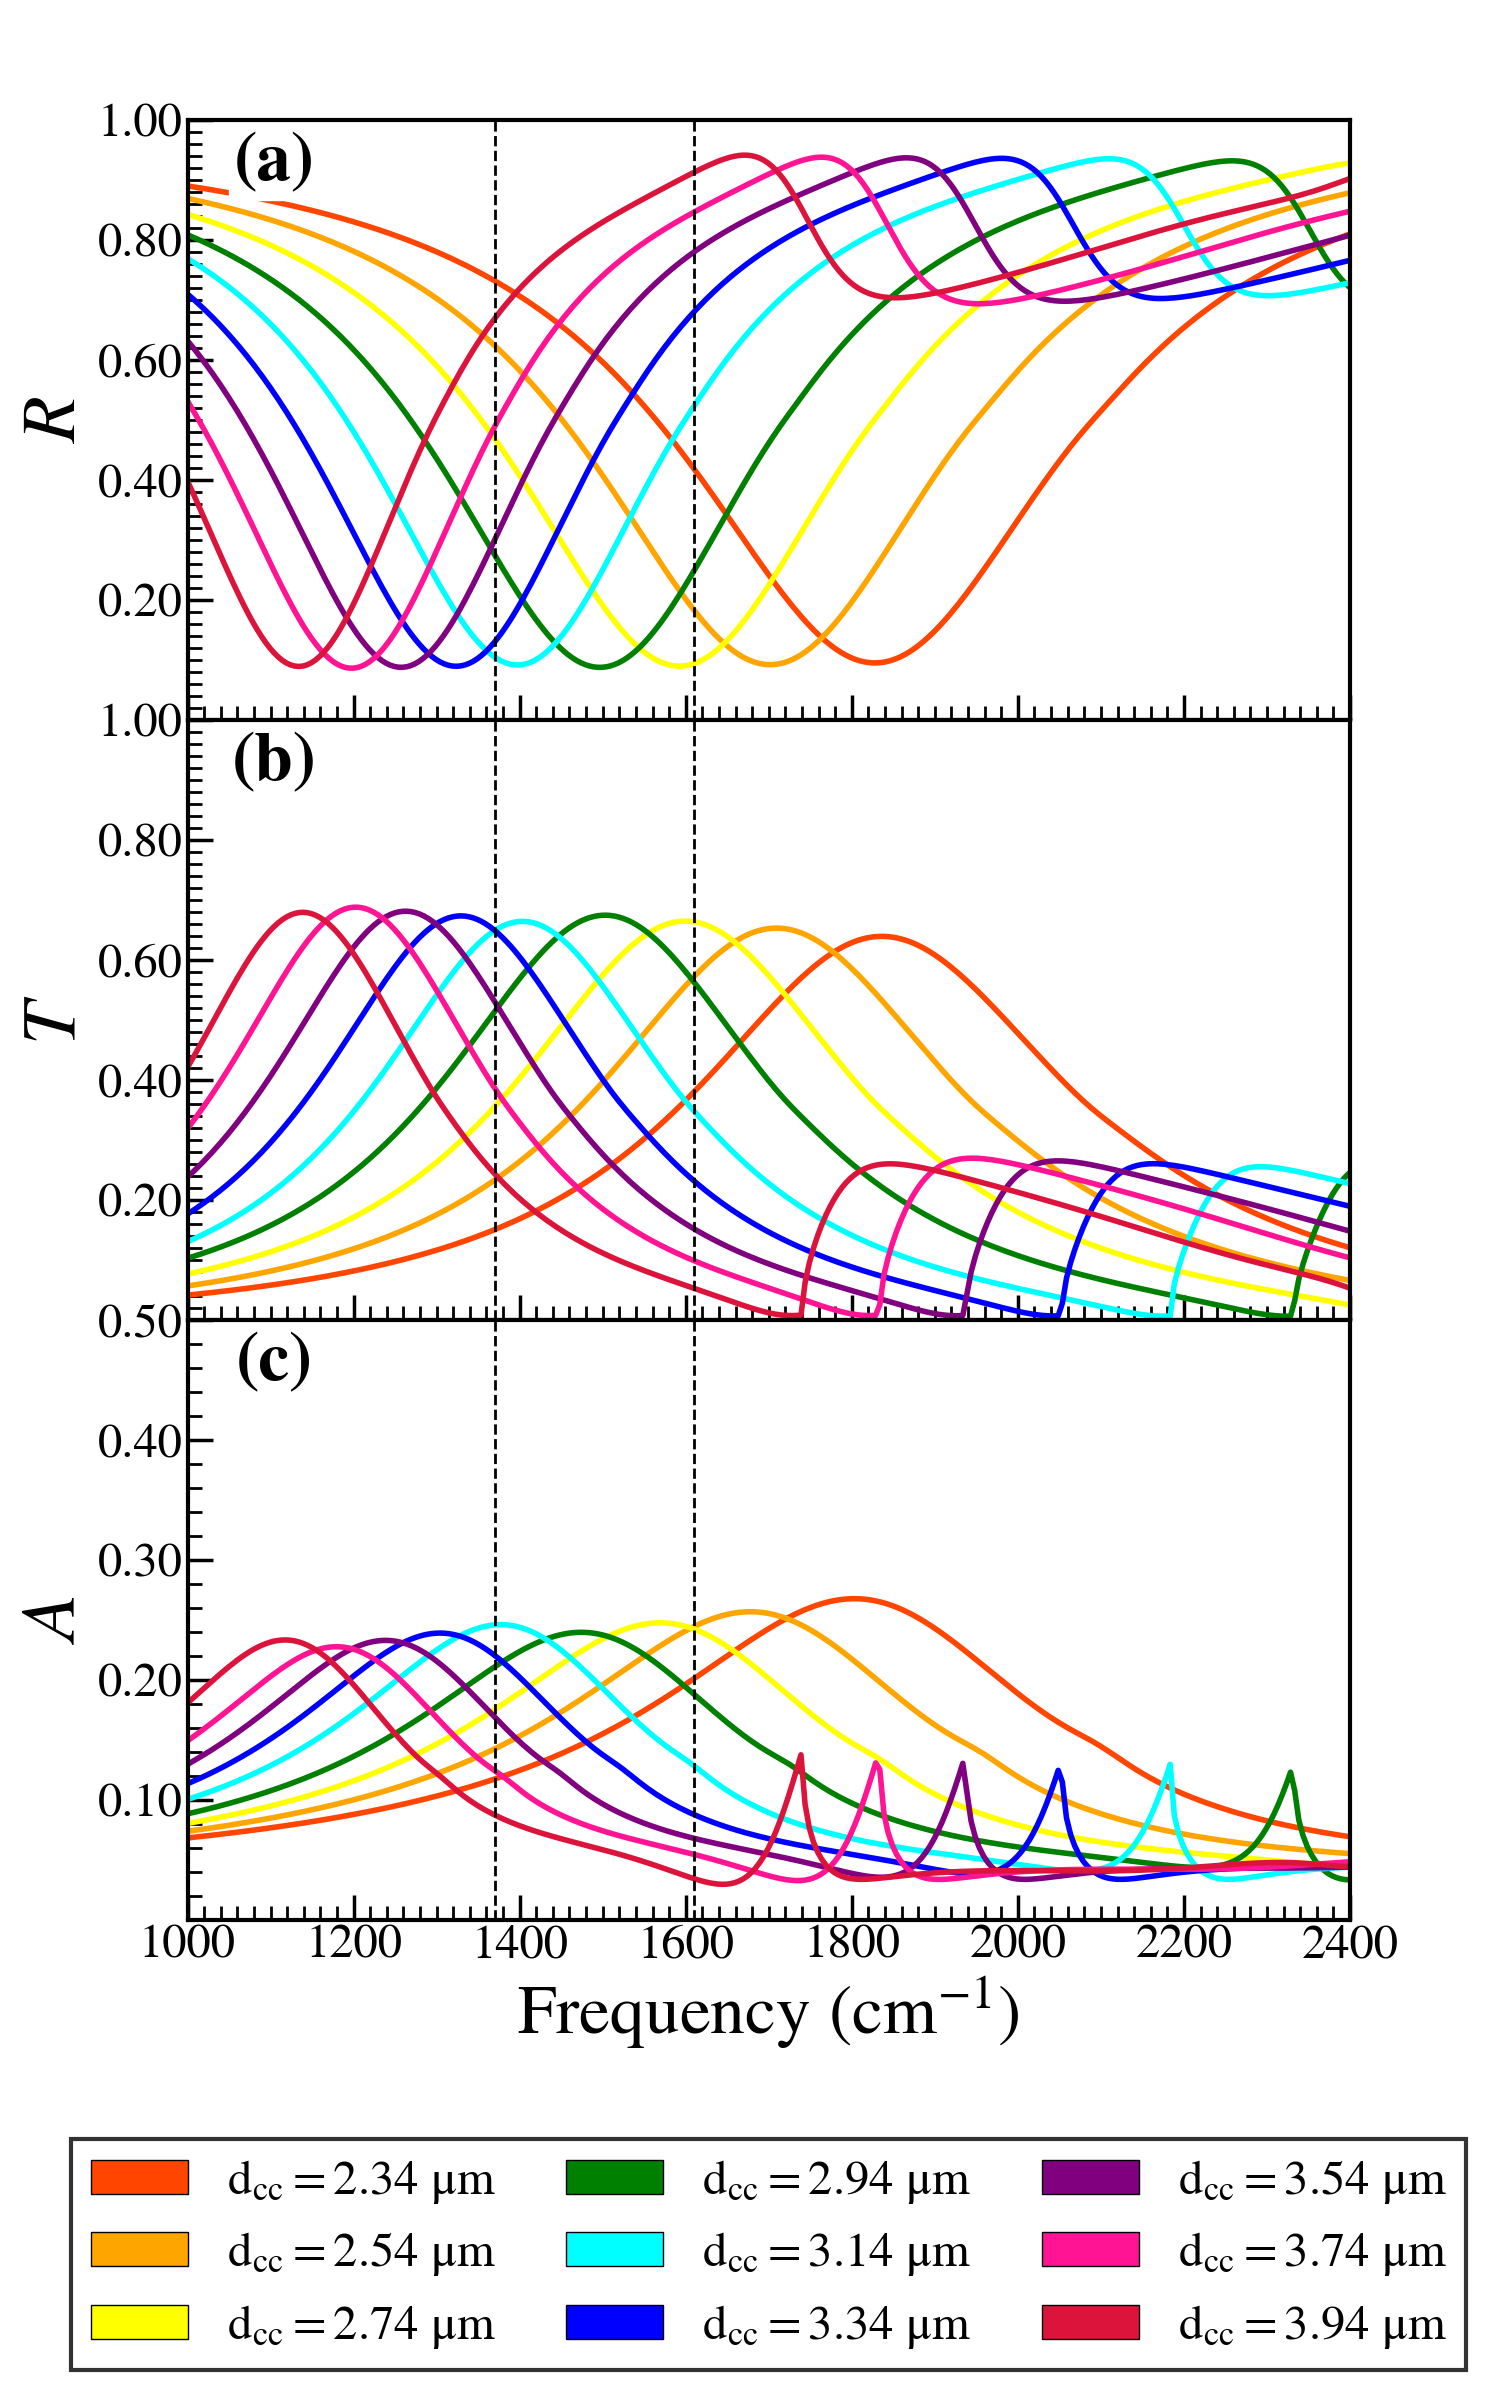
\includegraphics[width=0.45\textwidth]{Figures/UncRTA1000_2400.png}
			  \caption{The spectra for the UCDI at a range of $d_\mathrm{CC}$ values. (a) Reflectance spectra. (b) Transmittance spectra. (c) Absorptance spectra.  The vertical black dashed lines in this figure indicate the position of the hBN TO and LO phonon frequencies as described in \textcolor{cyan}{Chapter 2 [ref]}.}
			  \label{fig:3.3}
			\end{figure}
			
		\subsection{Coupled Device}
		\label{sec:CD}
			The equivelant CD data to those shown in sections~\ref{sec:BD} and~\ref{sec:UCDI} can be seen in Fig.~\ref{fig:3.4}. The most prominent effect observed in the CD is that the plasmon resonances split into two main peaks to either side of the hBN TO phonon frequency when compared to equivelant $d_\mathrm{CC}$ UCDI. The peaks for $d_\mathrm{CC} = 3.14\,\si{\um}$ device shifted approximately equal amounts above and below the hBN TO phonon frequency. As with the UCDI the resonances of the Rayleigh anomalies remained unchanged.

			Another notable feature that is observed in most of the absorptance spectra depicted in Fig.~\ref{fig:3.4} (c), is a small peak centered close to the hBN TO phonon frequency, which is also close to  the center of the absorptance peak of the non-plasmonic UCDII. Less obvious in these spectra, but also present are a series of small peaks and shoulders that lie between the hBN TO and LO frequencies, the nature of these latter features will be elucidated below.

			\begin{figure}[!htb]
			  \centering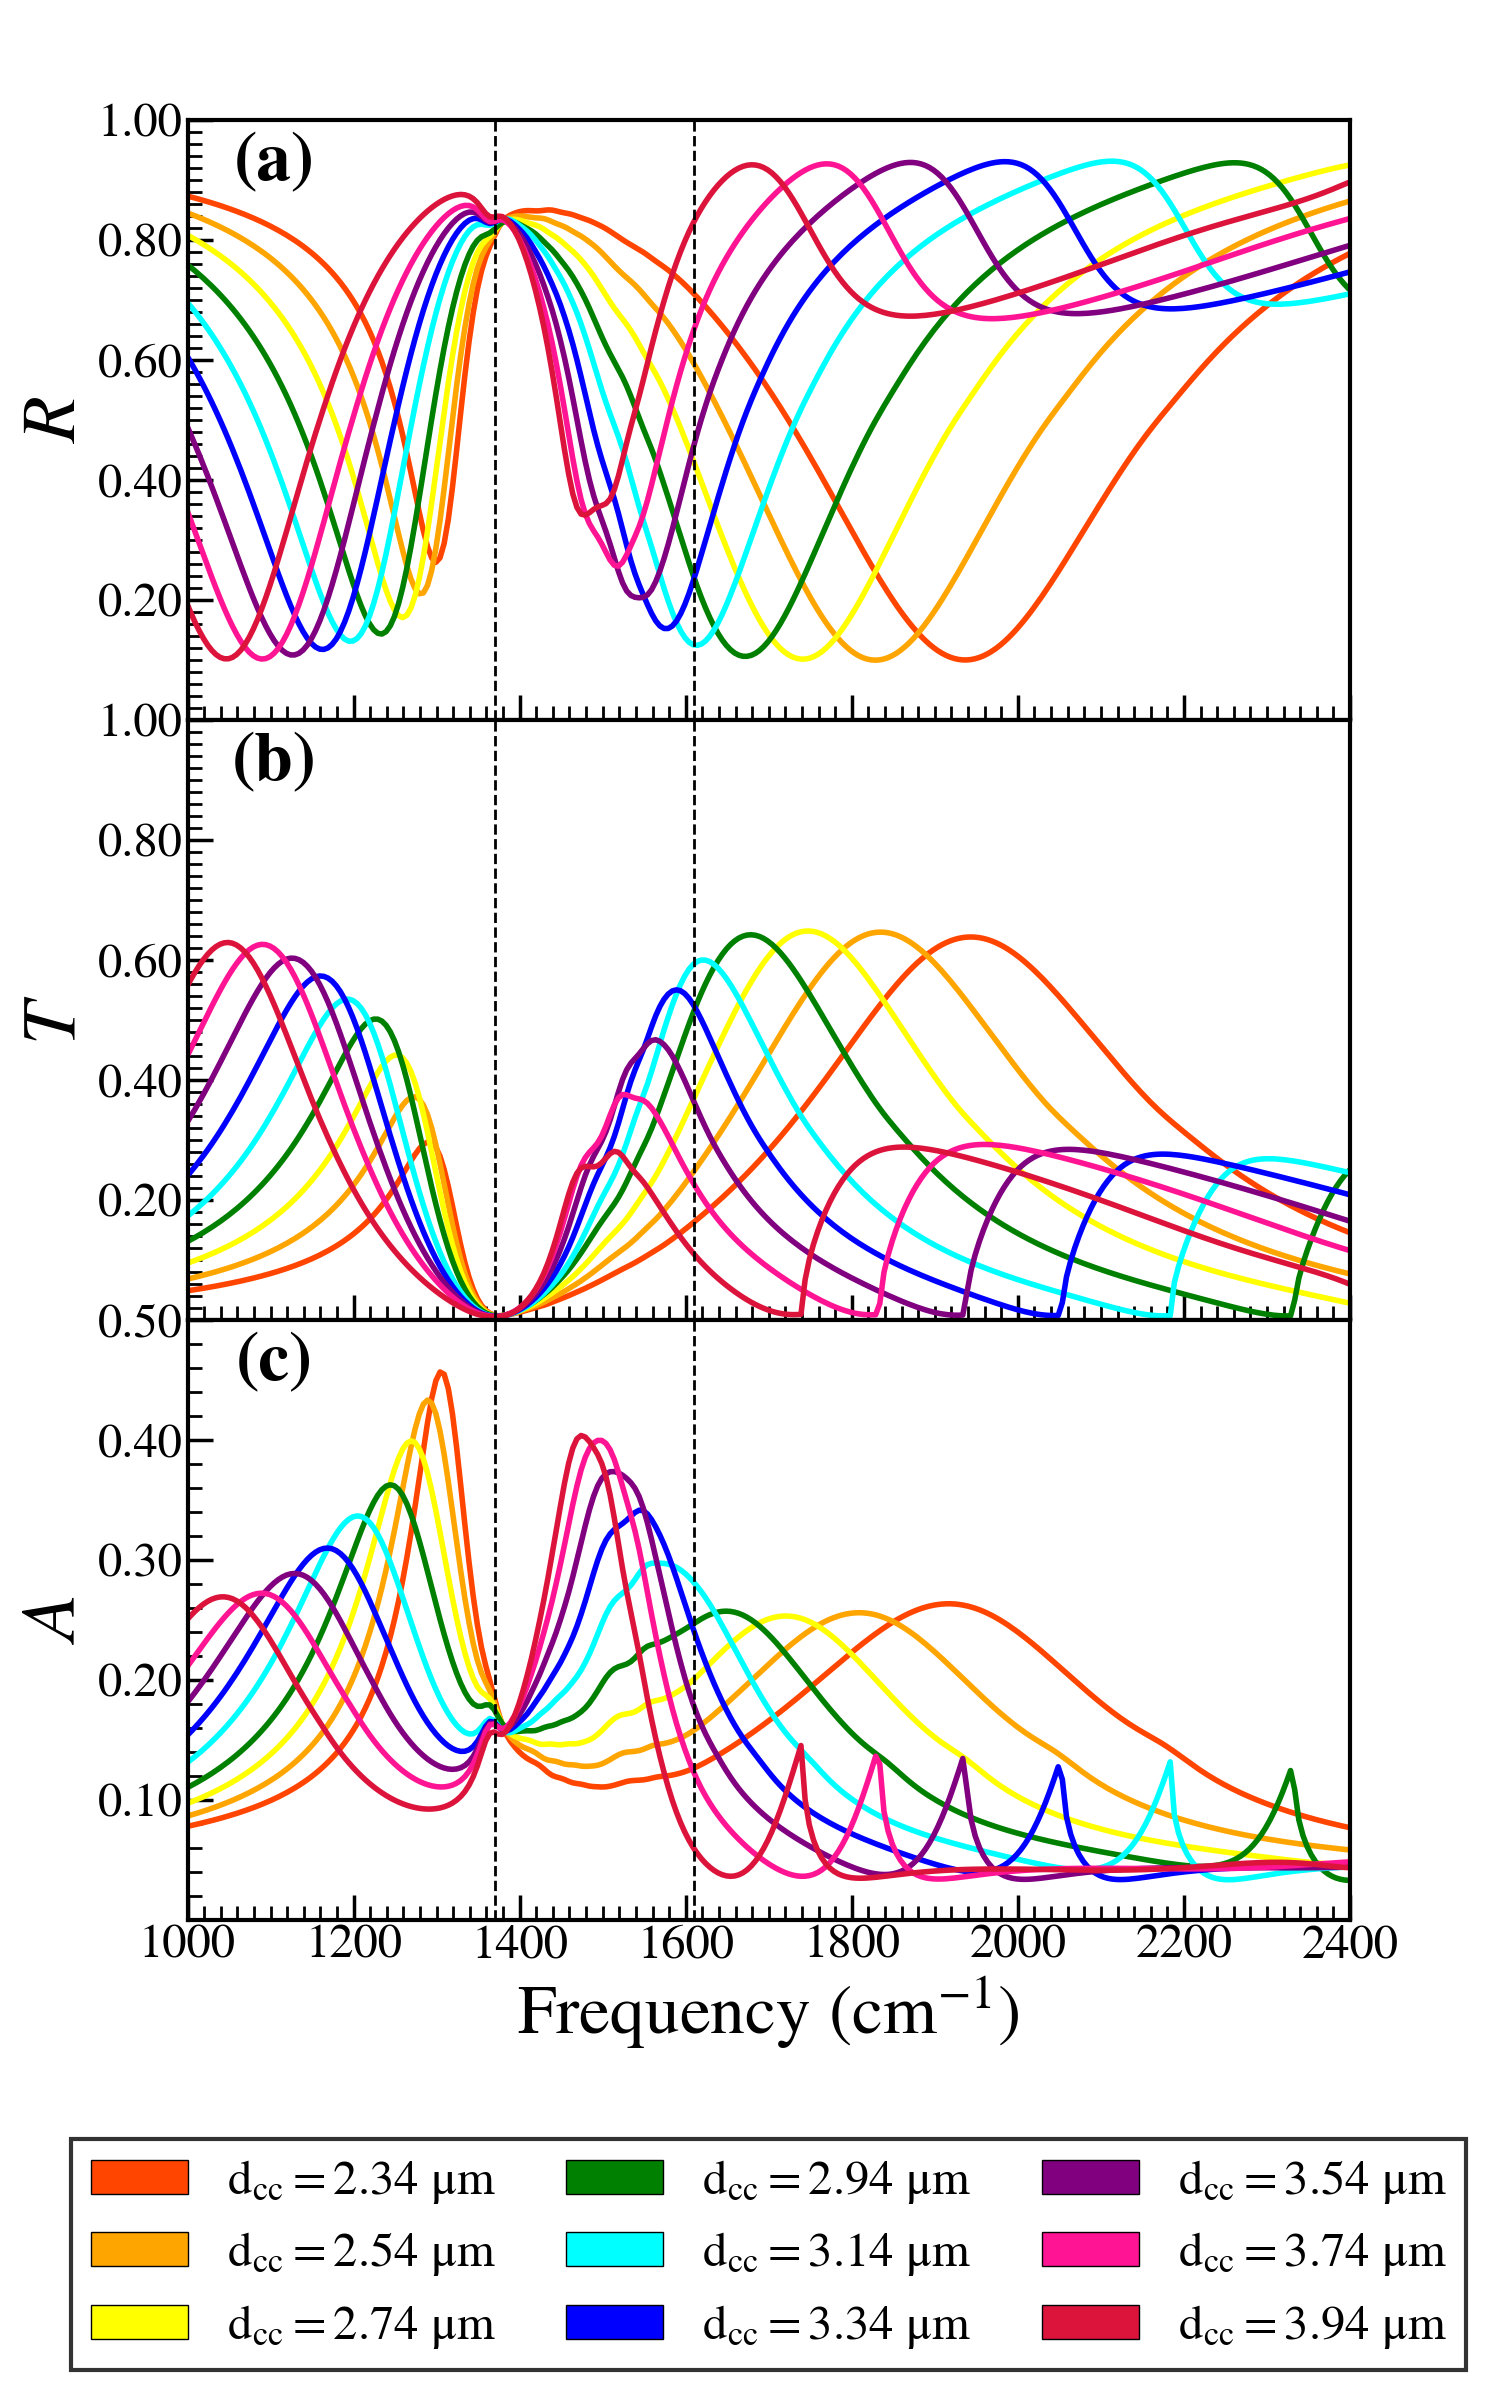
\includegraphics[width=0.45\textwidth]{Figures/FullRTA1000_2400.png}
			  \caption{The spectra for the CD at a range of $d_\mathrm{CC}$ values. (a) Reflectance spectra. (b) Transmittance spectra. (c) Absorptance spectra.  The vertical black dashed lines in this figure indicate the position of the hBN TO and LO phonon frequencies as described in \textcolor{cyan}{Chapter 2 [ref]}.}
			  \label{fig:3.4}
			\end{figure}


		\section{Validation}
		\label{sec:Val}

		\section{Peak Finding}
		\label{sec:PF}		
			To determine resonance values for various features it was necessary to perform peak finding. For plasmonic and Rayleigh resonances a naive nearest-neighbour peak finding algorithm was used for the resonances displayed in~\ref{fig:3.2}. To reduce use of computing rescources, an exponential function was fit to BD plasmonic resonances displayed in~\ref{fig:3.2}. From this relation the remaining resonances were calculated.  The data for this is shown in~\ref{fig:3.5}. 

			\begin{figure}[!htb]
			  \centering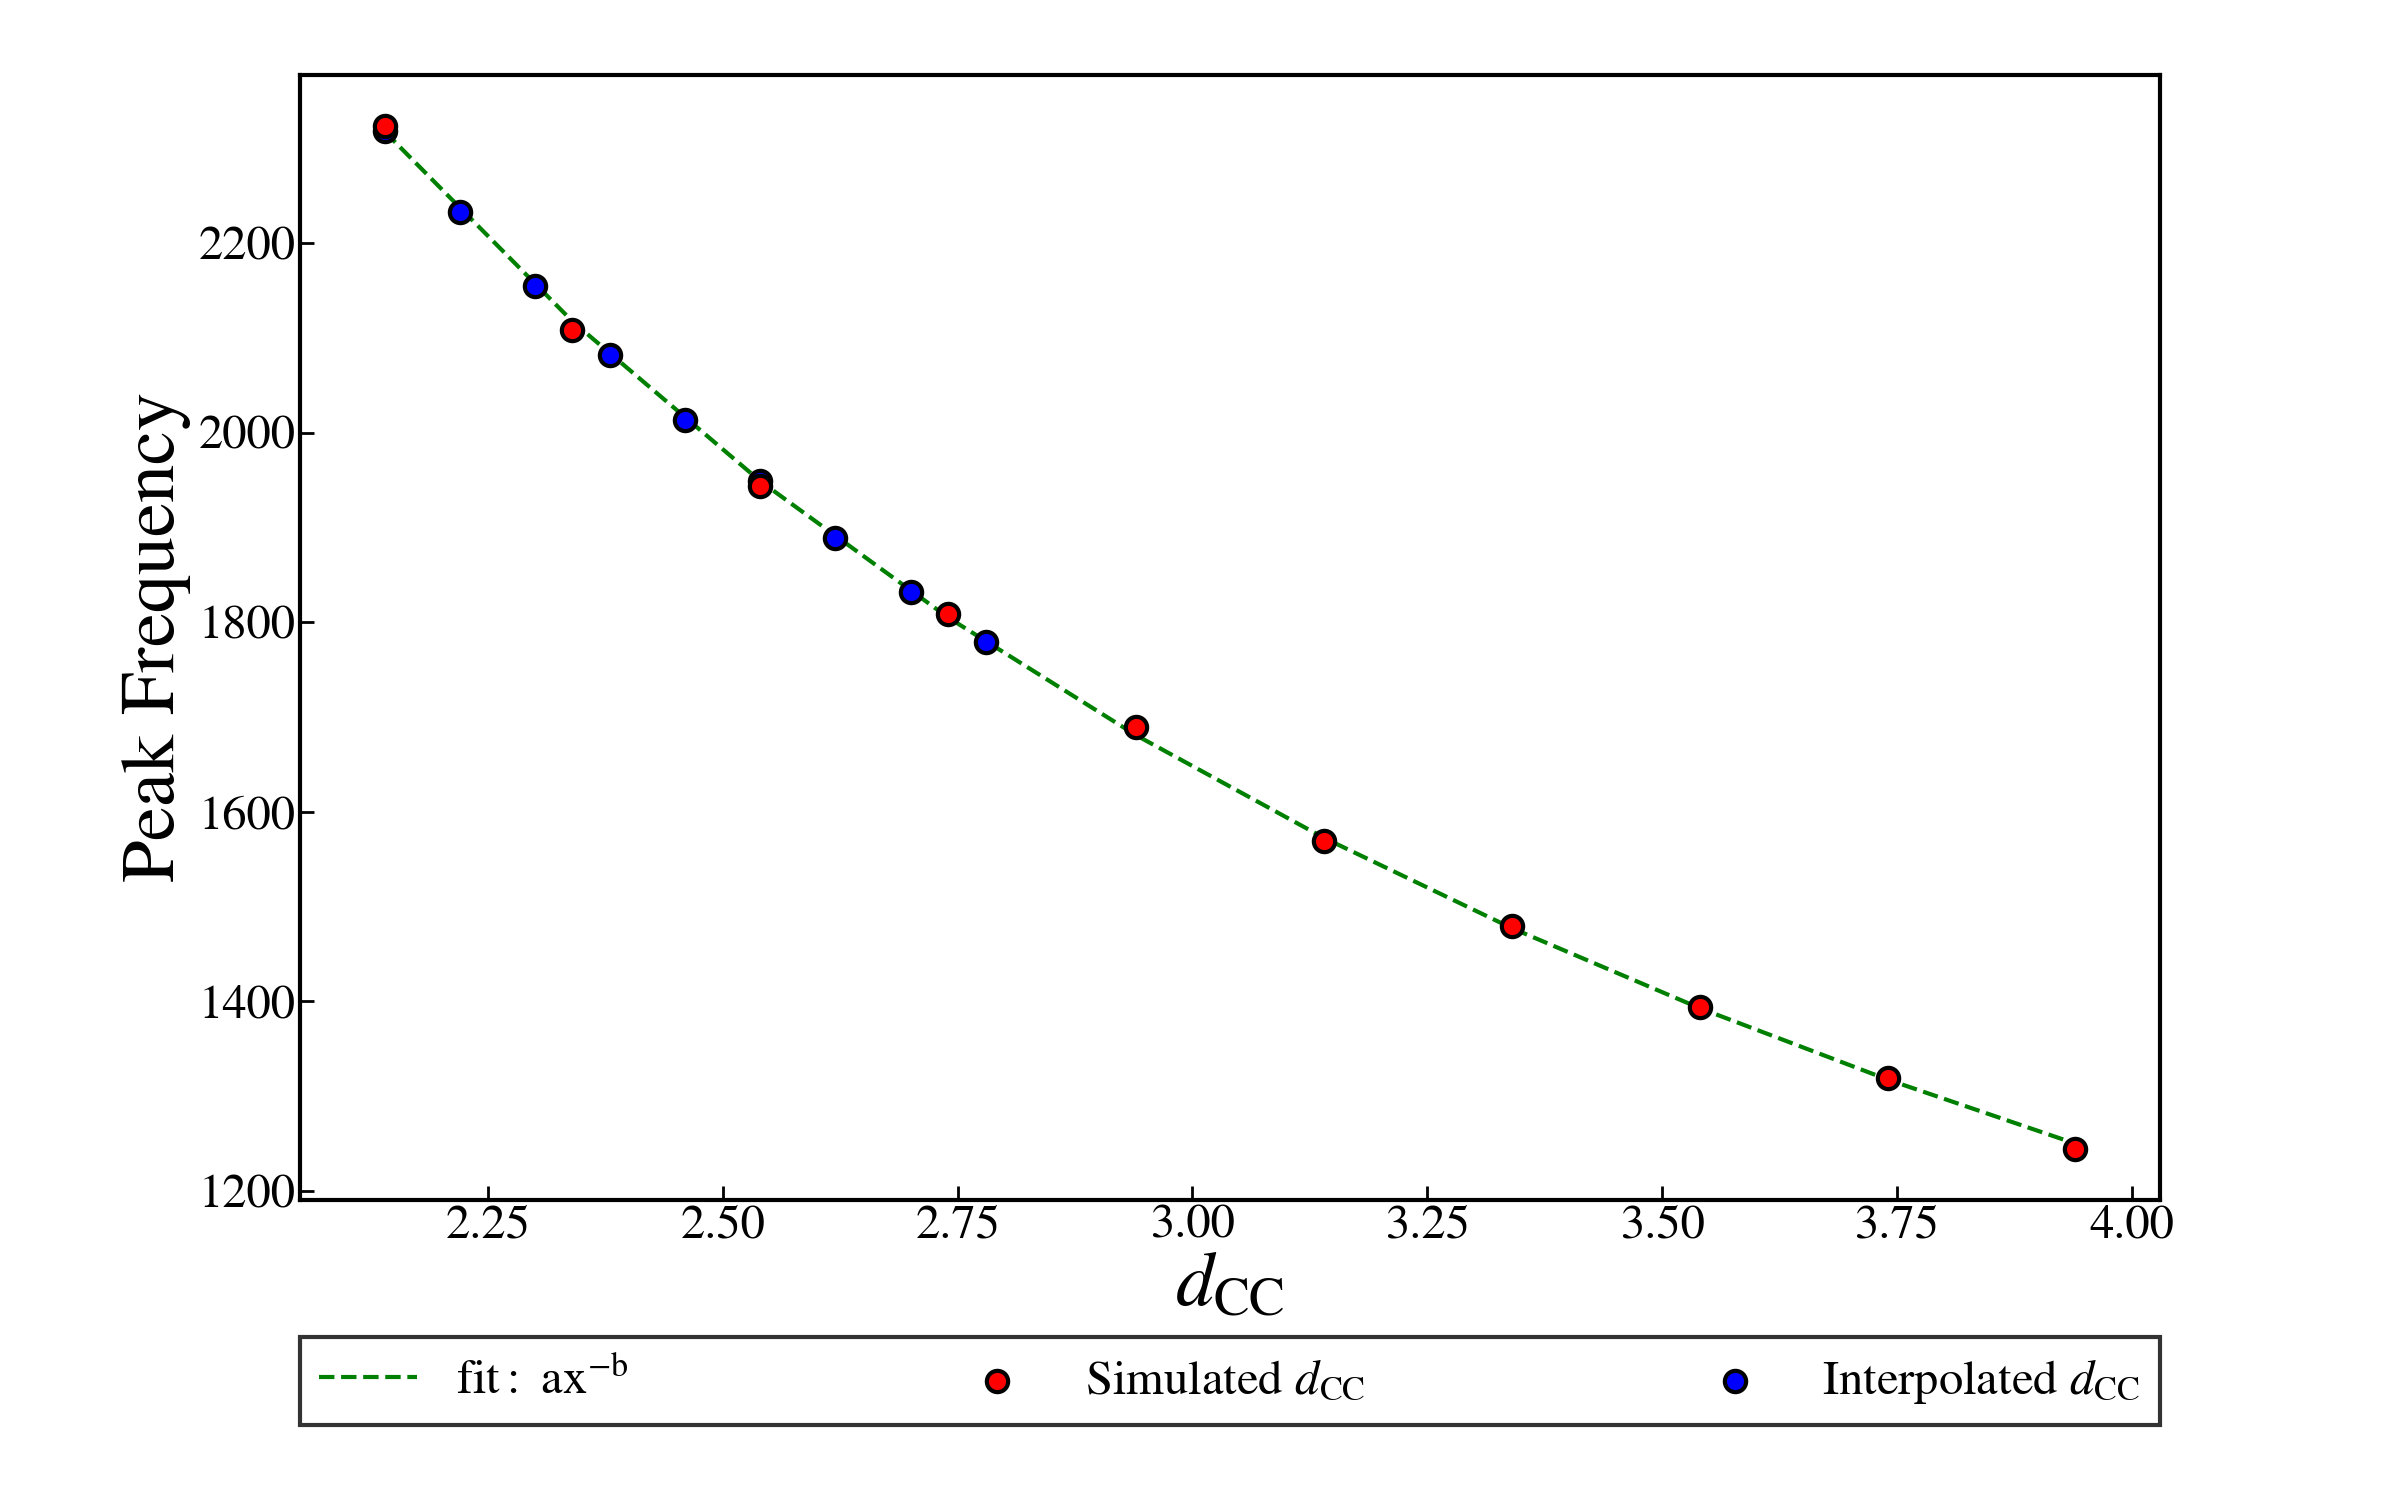
\includegraphics[width=0.85\textwidth]{Figures/NewDccvPeaksBare.png}
			  \caption{Bare device resonances calulated from a fit exponential curve of the $d_\mathrm{CC}$ BD plasmonic resonances.}
			  \label{fig:3.5}
			\end{figure}

			For the inflection points, seen within the Restrahlen band, the absorptance curve was twice differentiated with respect to frequency. The resulting curve was then multiplied by -1 and the same naive nearest-neighbour peak finding algorithm employed. To eliminate potentially spurious points a minimum $\frac{\partial A}{\partial \omega})$ value was used. Peaks below this value were discarded. This value was determined for each mode individually. The resulting values can be seen in~\ref{fig:3.6} for the $d_\mathrm{CC}=3.15 \si{\um}$ CD.


			\begin{figure}[!htb]
			  \centering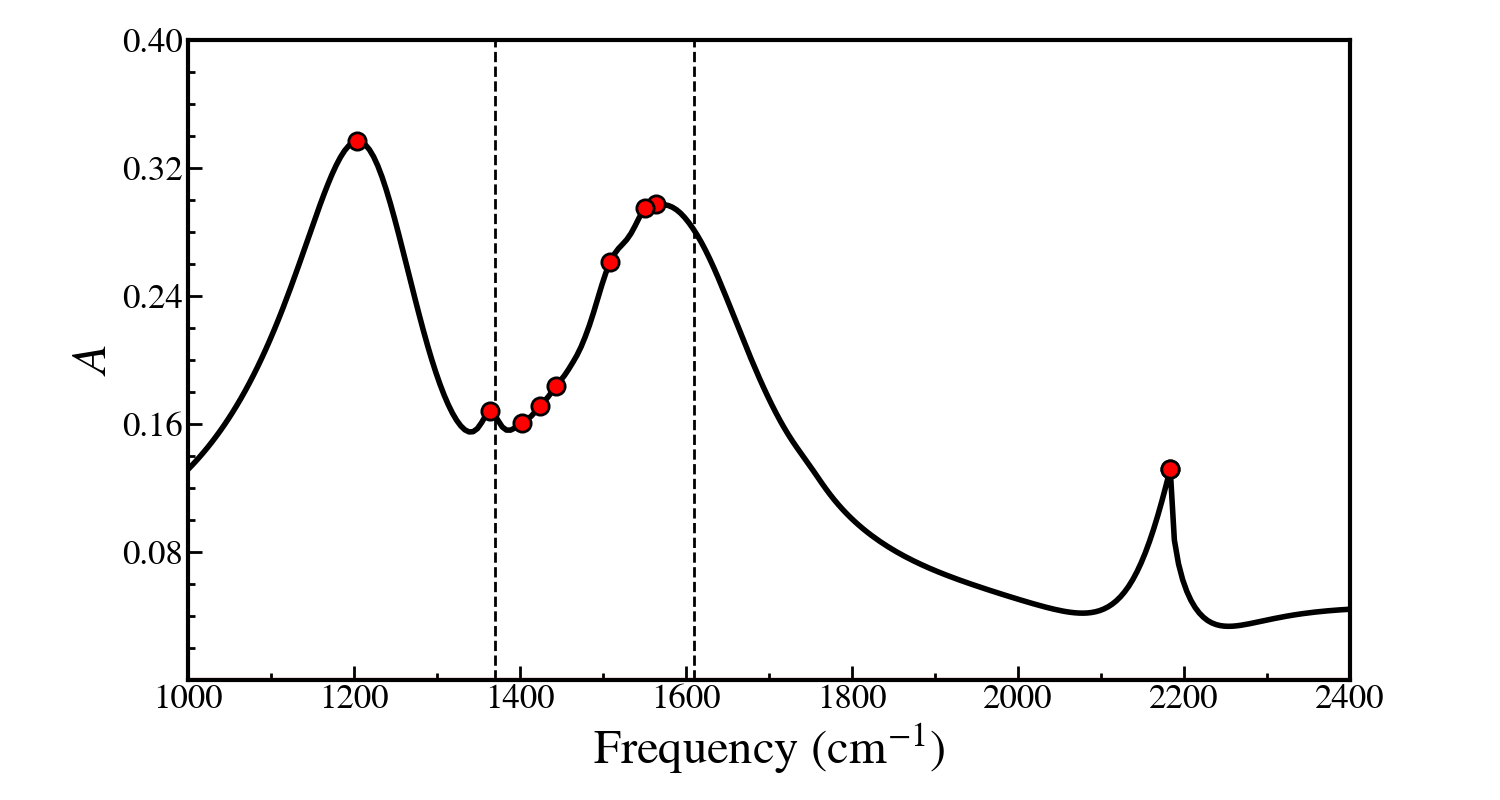
\includegraphics[width=0.85\textwidth]{Figures/NewAbsPeaksCrossSi1000_2400.png}
			  \caption{Modes locations for the $d_\mathrm{CC}=3.15 \si{\um}$ CD.}
			  \label{fig:3.6}
			\end{figure}
			
		\section{Far-Field Analysis}
		\label{sec:FFA}

			In order to investigate the effect of tuning the plasmon resonance through the hBN Restrahlen band, a series of FDTD simulations were performed at a range of distances between the nearest neighbor centers of the crosses, (\textit{i.e.,} $d_\mathrm{CC}$ in the range 2.34 -- 3.94 $\si{\um}$) and the absorptance spectra for the bare device (BD), the uncoupled device I (UCDI) and the coupled device (CD) structures were calculated from the frequency resolved Poynting vector data collected by the planar DFT sensors described in \textcolor{cyan}{Section (insert reference)}.  Fig.~\ref{fig:3.7} shows the absorption spectra calculated for all three devices. The vertical dashed lines in  Fig.~\ref{fig:3.7} indicate the positions of the hBN TO and LO phonons at 1360 and 1614 $\mathrm{cm}^{-1}$, respectively. The absorption spectrum of an $80\,\si{\nm}$ thick free-standing hBN film \textcolor{cyan}{(Reference)} is resonant with the TO phonon frequency. As can be seen from Fig.~\ref{fig:3.7} (b), the UCDI structure with $d_\mathrm{CC} = 3.14\,\si{\um}$ exhibits a plasmon absorptance peak that is most closely resonant with the hBN TO phonon and this device is the one studied most extensively in this chapter.

			Fig.~\ref{fig:3.7} (c) shows the absorption spectra for a series of CDs for a range of  $d_\mathrm{CC}$. Also shown in Fig.~\ref{fig:3.7} (c) is the absorptance spectrum of the UCDII with $d_\mathrm{CC} = 3.14\,\si{\um}$ (gray dotted line), which exhibits a single peak centered close to the hBN TO frequency. The most prominent effect observed in the CD is that the plasmon absorption spectra in UCDI split into two main peaks either side of the hBN TO phonon frequency, with the peaks for $d_\mathrm{CC} = 3.14\,\si{\um}$ device being shifted approximately equal amounts above and below the hBN TO phonon frequency.

			Another notable feature that is observed in most of the absorptance spectra depicted in Fig.~\ref{fig:3.7} (c), is a small peak centered close to the hBN TO phonon frequency, which is also close to  the center of the absorptance peak of the non-plasmonic UCDII. Less obvious in these spectra, but also present are a series of small peaks and shoulders that lie between the hBN TO and LO frequencies, the nature of these latter features will be elucidated below.  

			Finally, there are a series of cusps that occur in the spectra of all three devices, only one of which is shown in Fig.~\ref{fig:3.7}. This feature occurs at a frequency of $\sim 1750\,\mathrm{cm}^{-1}$ for all three $d_\mathrm{CC} = 3.94\,\si{\um}$ devices. The assignment of these latter features will be deferred until later in this chapter.

			\begin{figure}[!htb]
			  \centering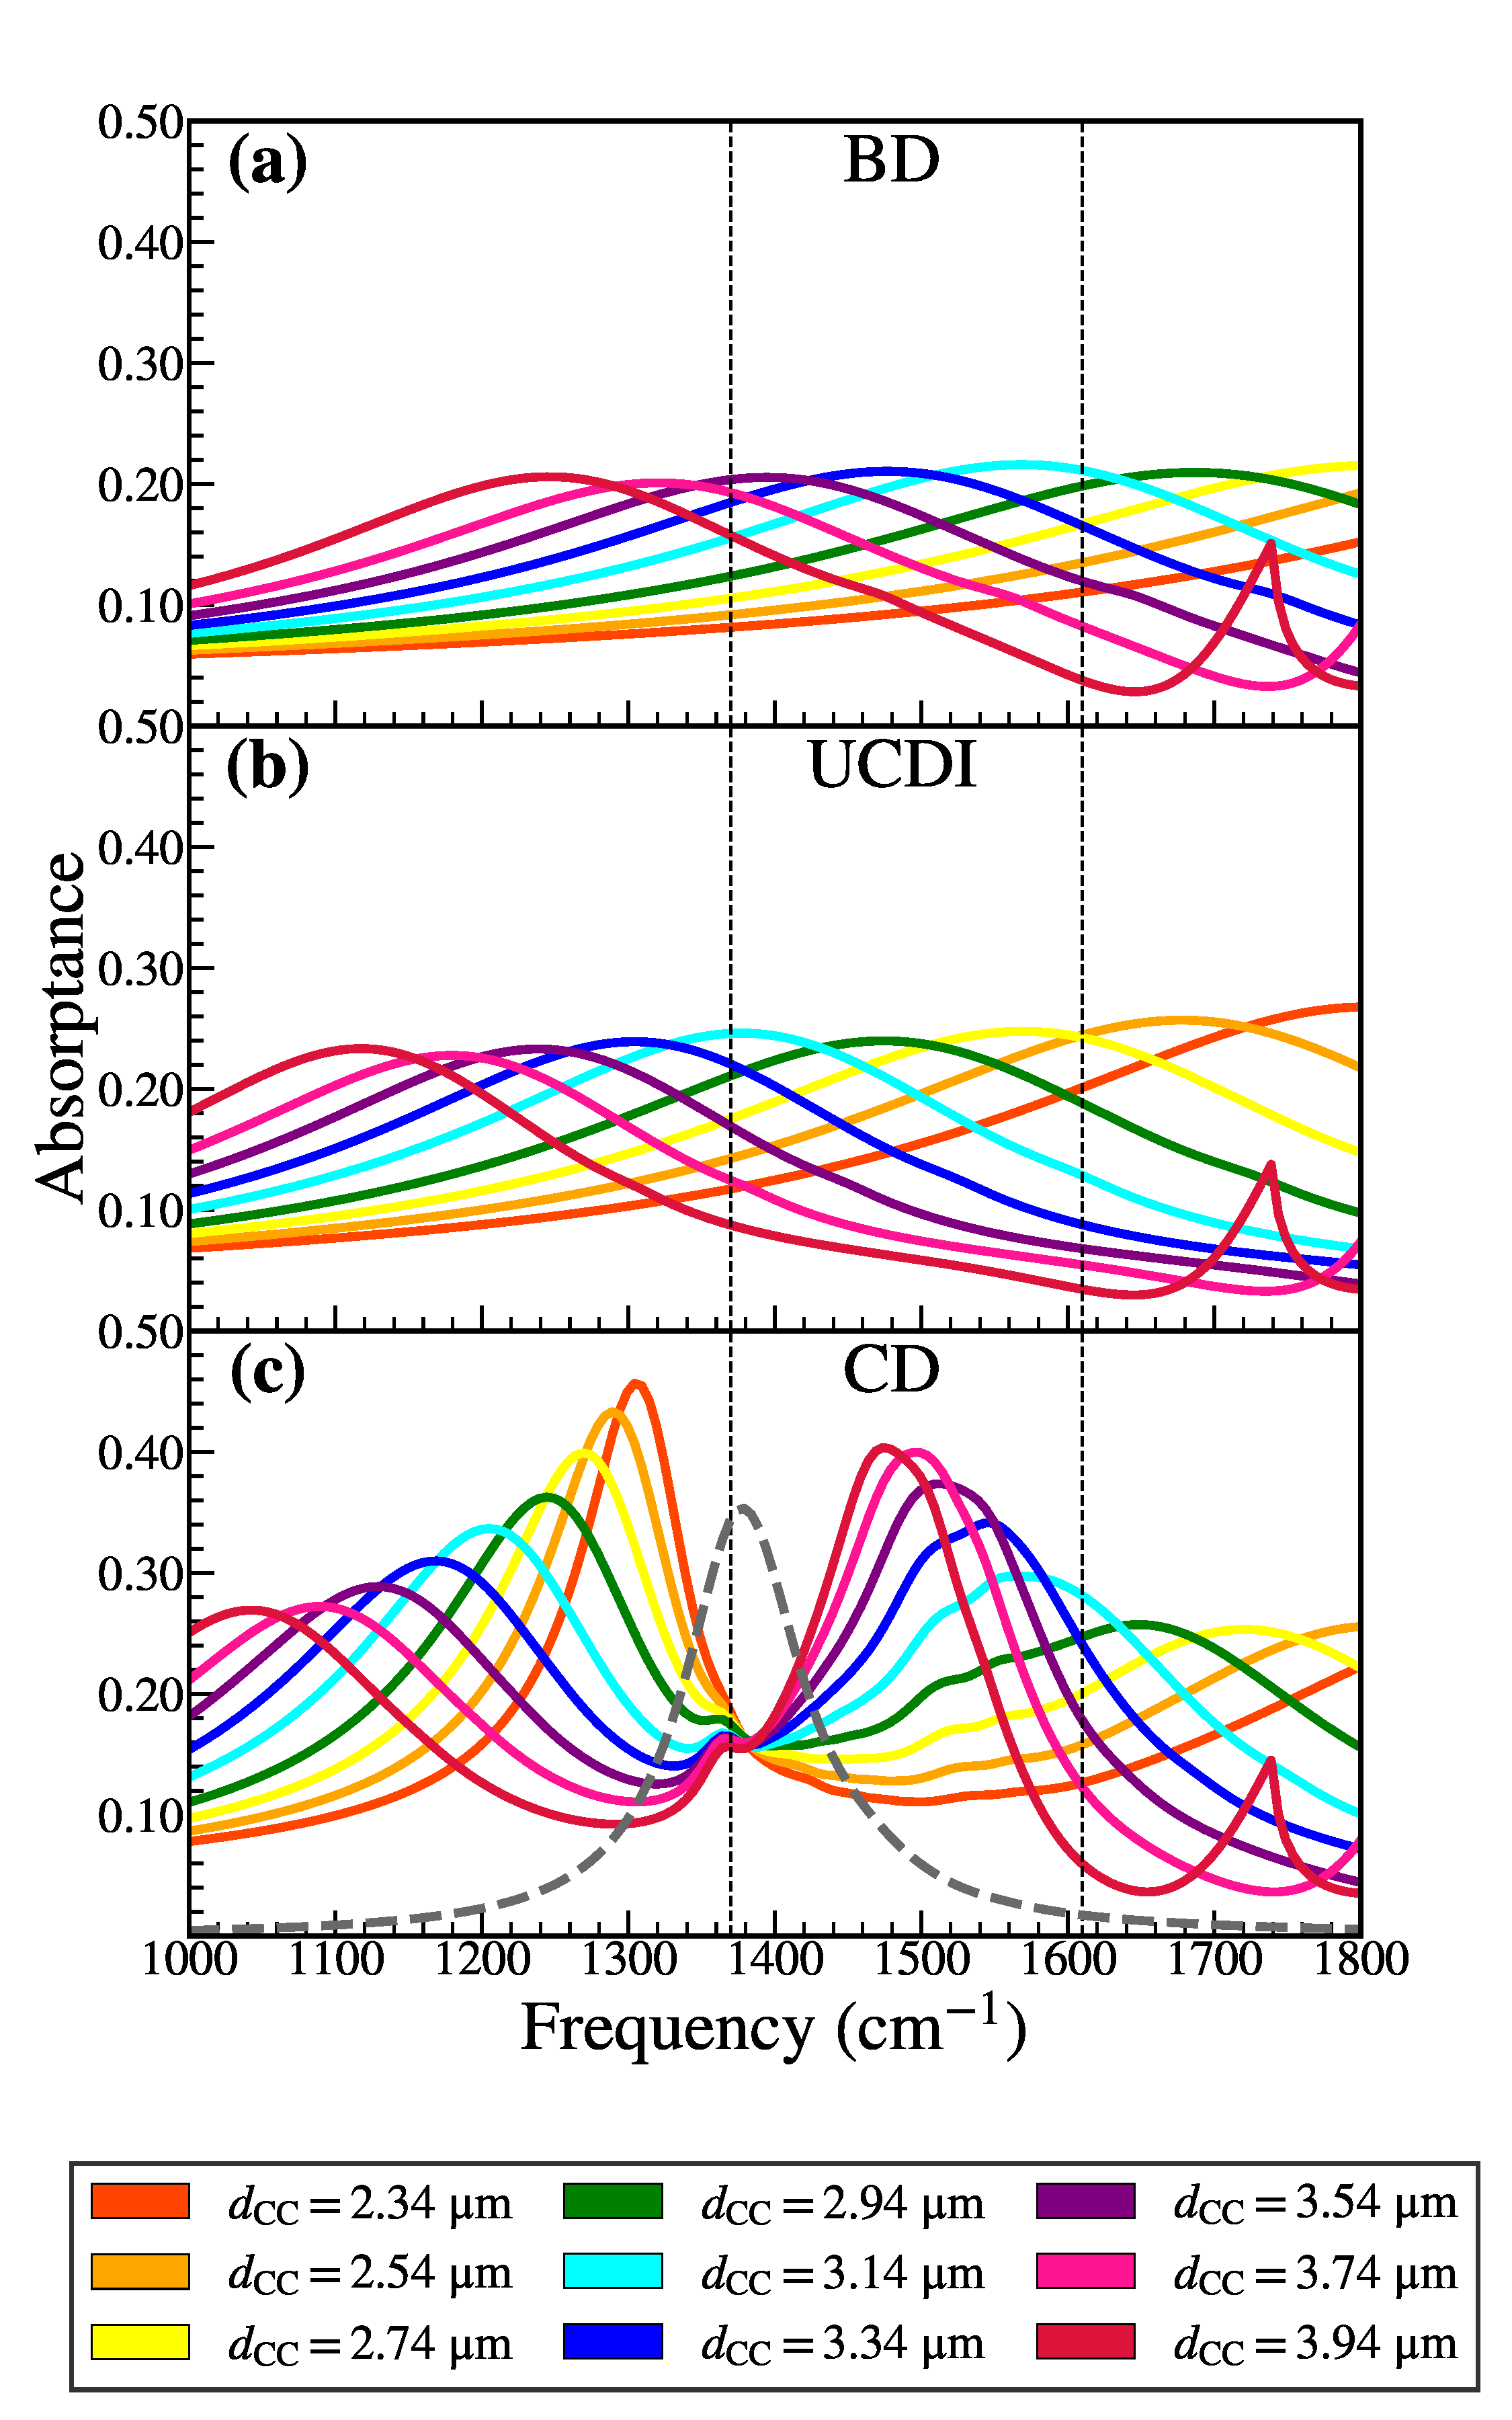
\includegraphics[width=0.5\textwidth]{Figures/Fig2.pdf}
			  \caption{(a) The absorptance spectrum of the BD for a range of $d_\mathrm{CC}$ values. (b) The absorptance spectra of the UCDI. (c) The absorptance spectra of the CD. The gray dotted curve in pane (c) depicts the absorption spectra for the UCDII with $d_\mathrm{CC} = 3.14\,\si{\um}$.  The vertical black dashed lines in this figure indicate the position of the hBN TO and LO phonon frequencies as described in the main text.}
			  \label{fig:3.7}
			\end{figure}

			In order to better analyze the absorptance peak frequency shifts observed in Fig.~\ref{fig:3.7}, the data in Fig.~\ref{fig:3.7}(b) and (c) were plotted in colormap form as a function of $\nu_\mathrm{bare}$ as prescribed in Wan \textit{et al.} \cite{Wan:16} in Fig.~\ref{fig:3.8}(a) and \ref{fig:3.8} (b) respectively. These plots can act as a proxy for the dispersion curves, although with some limitations. The peak positions in the absorptance spectra were determined using a simple peak fitting algorithm \cite{peakfinding} and plotted on top of the colormaps. In both Fig.\ref{fig:3.8} (a) and (b), the peaks in the spectra indicated by the orange, green and blue triangles are due to Rayleigh anomalies \cite{Wood:1902,Rayleigh:1907,Gao:2009} with indices (0,1), (1,1), (0,2), and their symmetric counterparts, respectively. The red squares in Fig.~\ref{fig:3.8}(a) indicate the main absorptance peak due to the plasmon-polariton in the UCDI. These peaks track linearly with $\nu_\mathrm{bare}$, the peak of the absorptance of corresponding BD and is analogous to the reflection data presented by Wan \textit{et al.} \cite{Wan:16} in their Fig. 3(a). The red squares in Fig.~\ref{fig:3.8}(b) show how the absorptance peak due to the plasmon-polariton in UCDI splits due to the interaction the bulk phonon-polariton in the hBN. The circles in Fig.~\ref{fig:3.8}(b) are interpreted as indicating slab phonon-polariton modes in the hBN layer; this interpretation will be further supported by the near-field data below.

			\begin{figure}[!htb]
			  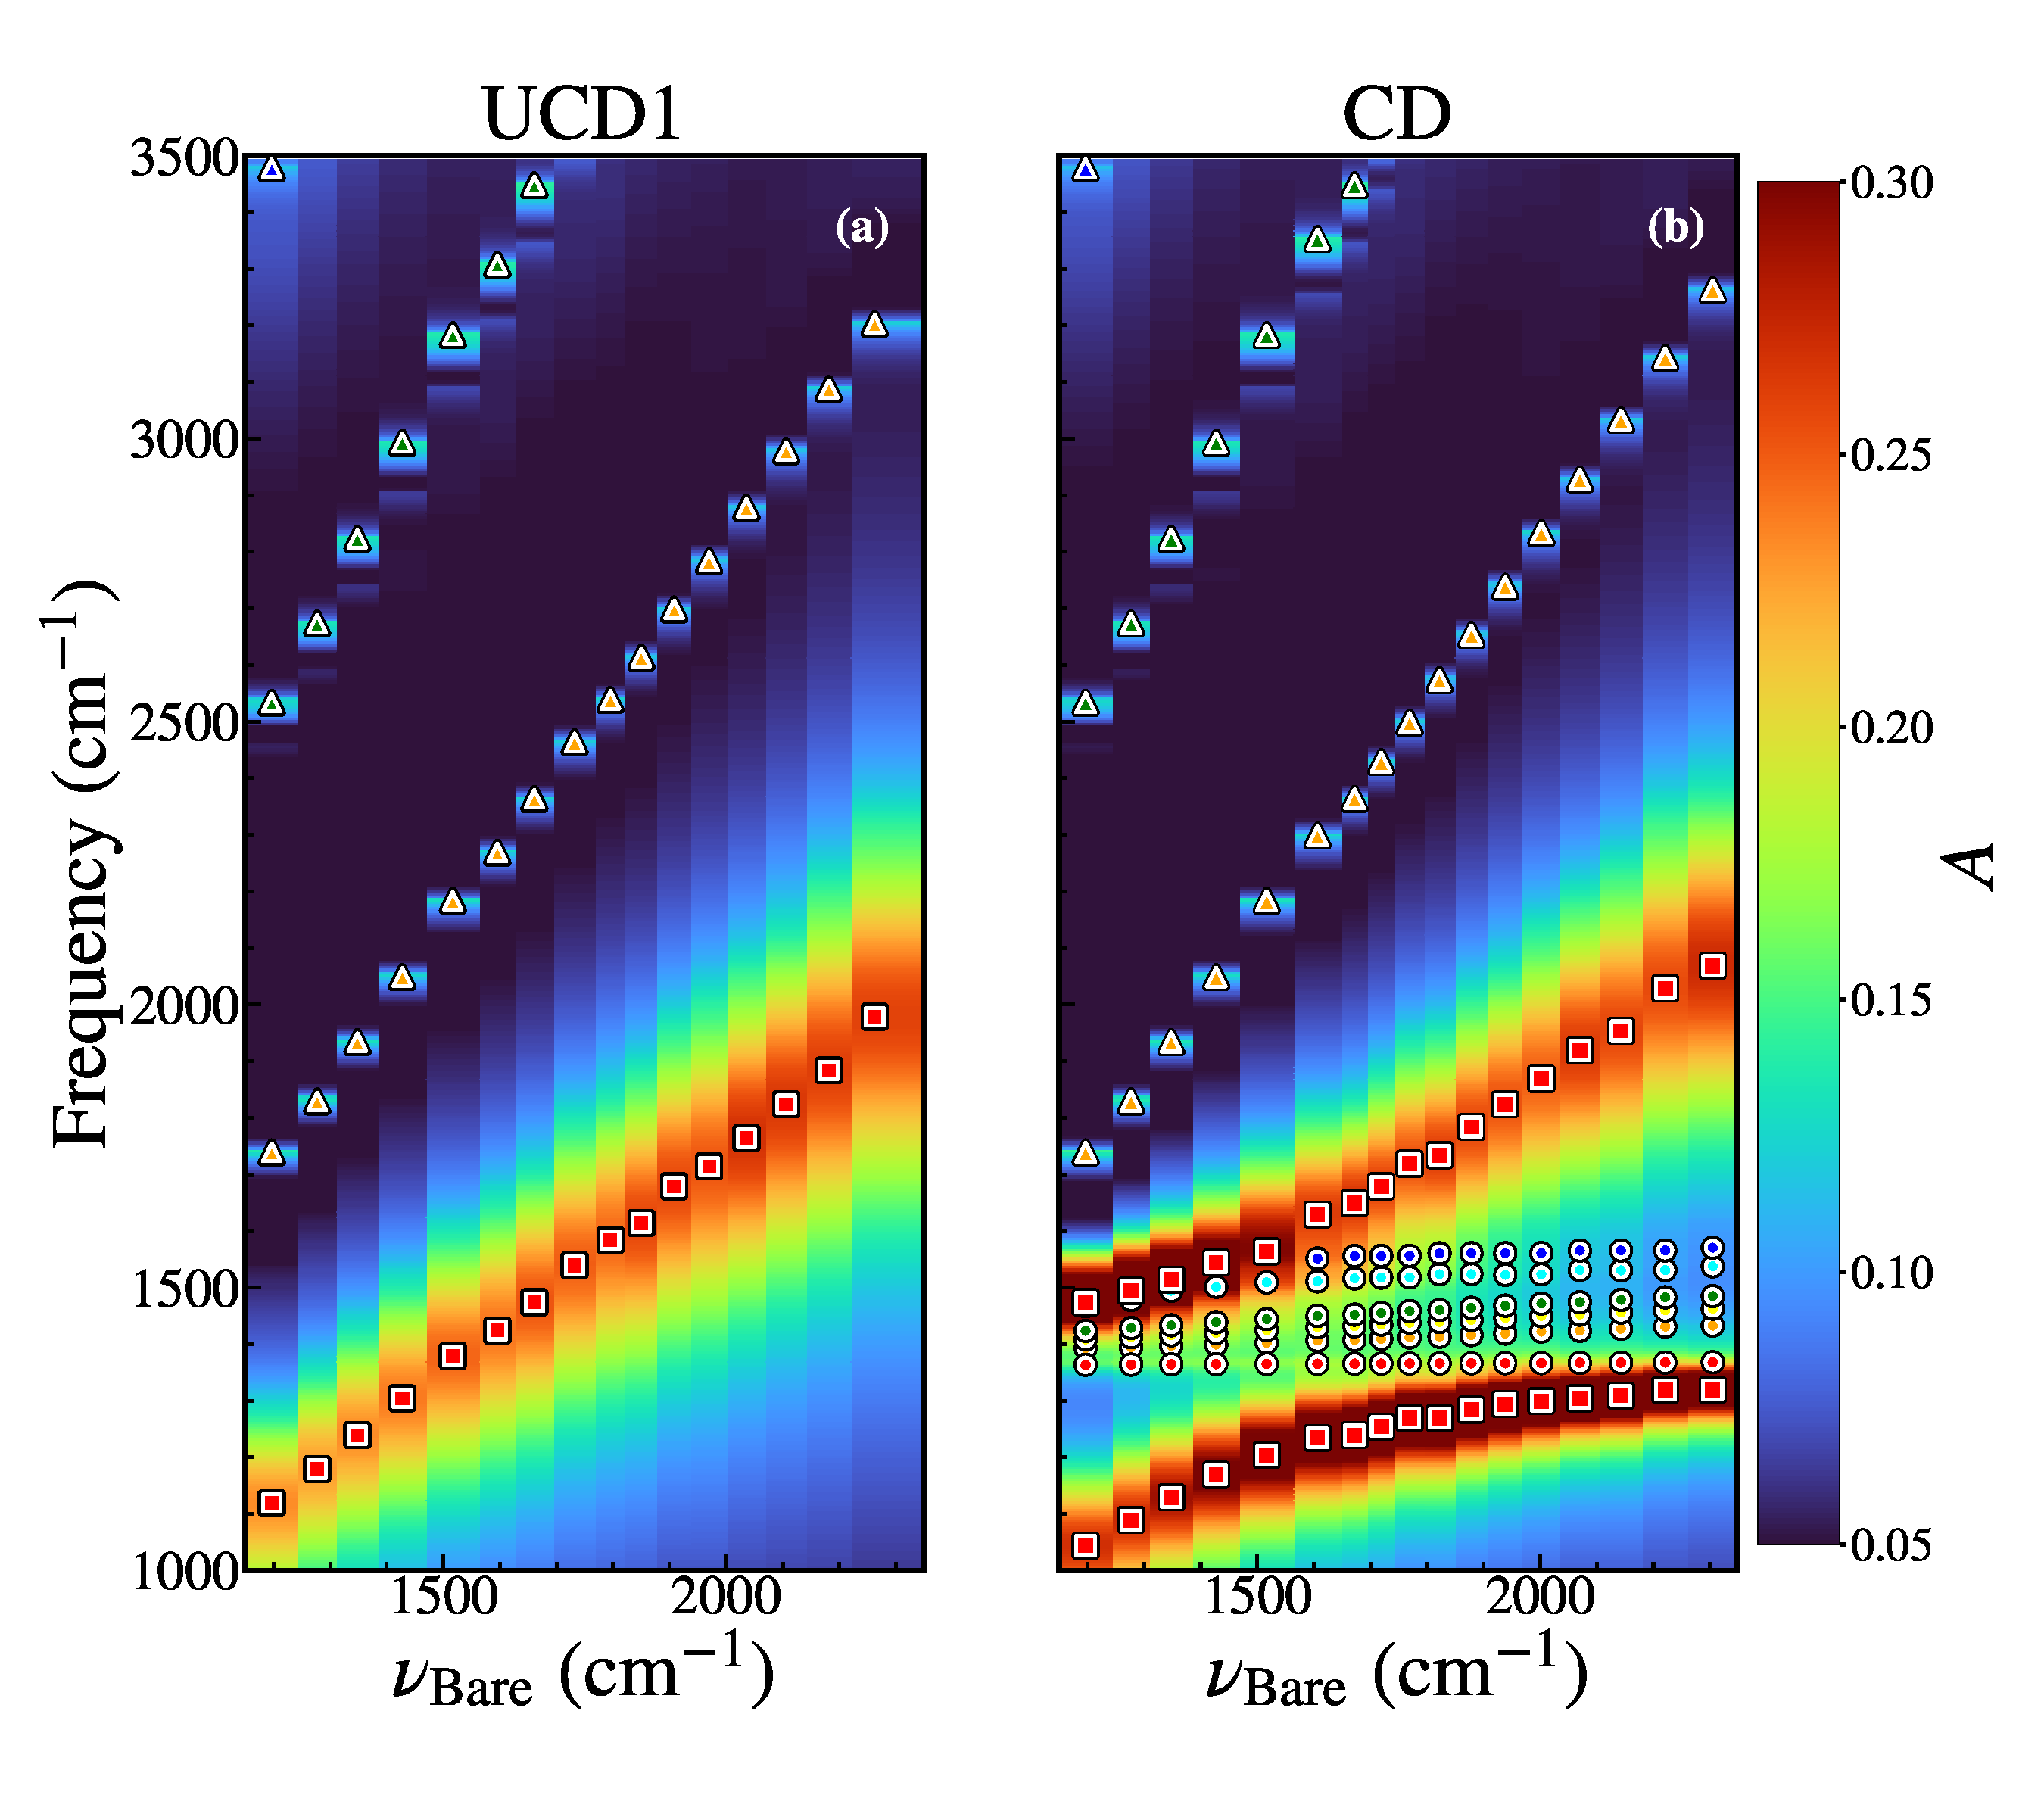
\includegraphics[width=0.75\textwidth]{Figures/Fig3.pdf}
			  \caption{(a) Absorptance spectra for the UCDI vs the peak frequency of the BD ($\nu_\mathrm{bare}$) plotted as a color map. The symbols indicate the peaks in the absorptance spectra. The triangular symbols are due to Rayleigh anomalies, while the square symbols indicate the plasmon-polariton, which shifts linearly with $\nu_\mathrm{bare}$.
			    (b) Absorptance spectra for the CD vs the peak frequency of the BD ($\nu_\mathrm{bare}$) plotted as a color map. The symbols indicate the peaks/shoulders in the absorptance spectra. The triangular symbols are due to Rayleigh anomalies, while the square symbols show the interaction between plasmon-polariton in the nanopatterned Au film and the bulk phonon-polariton in the hBN. The interpretation of the features labeled by the circular symbols are given in the main text.}
			  \label{fig:3.8}
			\end{figure}

		\section{Near-Field Colormap Data}
		\label{sec:NFAI}
				In order to gain insight into the coupling between the plasmon-polaritons in the nanopatterned Au and the phonon-polaritons in hBN film, the electric field distributions, $|\bm{E}|$, at the position of the vacuum/hBN interface were investigated for all four devices,  \textit{i.e.,} BD, UCDI, UCDII, and CD, as shown in Fig.~\ref{fig:3.9}. This position was selected as these field distributions are accessible to experimental techniques. In order to gain additional insight, the cross-sectional field maps (which are not accessible experimentally) are also shown in Fig.~\ref{fig:3.9} directly below the corresponding planar data. Fig.~\ref{fig:3.9} presents data after $y$-polarized excitation at three different frequencies, \textit{i.e.,} below the hBN restrahlen band at $\nu = 1200 \, \mathrm{cm}^{-1}$, within the hBN restrahlen band at $\nu = 1500 \, \mathrm{cm}^{-1}$ and above the restrahlen band at $\nu = 1700 \, \mathrm{cm}^{-1}$. The data excited at frequencies above and below the restrahlen band is expected to be predominantly plasmonic in nature for   BD, UCDI and CD; this is borne out by the data in Fig.~\ref{fig:3.9} (a)--(h) and (q) -- (x), respectively. In particular, in the case of the BD, there are field hot-spots at the inner corners of the cross pattern. In both the UCDI and CD, these hot spots are reproduced and smeared out; in the case of the CD this is due the presence of the  hBN capping layer. The UCDII exhibits no evidence of field hot-spot behavior as expected for a structure without a nanostructured metallic layer. It is noticeable that in all the above cases the only rapid variations in the field take place right at the boundary between the metal/dielectric cross and the enclosed vacuum. Based upon the above discussion, the field maps shown in panes (b) and (r) of Fig.~\ref{fig:3.9} are taken to be a prototypical signature of plasmonic behavior in the capped devices considered in this paper. In the case of the CD, see Fig.~\ref{fig:3.9} (d) and (t), the field maps are very similar to those depicted in Fig.~\ref{fig:3.9} (b) and (r), indicating that the behavior observed is predominately plasmonic when this device is excited either above or below the hBN restrahlen band.

				Excitation of the above devices within the hBN restrahlen band at $\nu = 1500 \, \mathrm{cm}^{-1}$ reveals significantly different behavior. In the case of the BD and UCDI, the planar, Fig.~\ref{fig:3.9} (i) and (j), and cross-sectional field maps, Fig.~\ref{fig:3.9} (m) and (n), strongly resemble the plasmonic field maps excited outside the restrahlen band, in particular those excited at $\nu = 1700 \, \mathrm{cm}^{-1}$. The UCDII planar field map, Fig.~\ref{fig:3.9} (k), exhibited high spatial frequency variations in the $y$-direction in the region within the cross, although there is comparatively little high spatial frequency variation in the $x$-direction. This behavior is reproduced outside the cross, but at a noticeably different spatial frequency. An examination of the cross-sectional field map, Fig.~\ref{fig:3.9} (o), reveals that there is a guided slab mode within the hBN layer of this device. The CD planar field map, Fig.~\ref{fig:3.9} (l), exhibited high spatial frequency variations in both the $x$- and $y$-directions in the regions within and outside the cross. The contrast of these spatial variations is somewhat greater than that observed in Fig.~\ref{fig:3.9} (k). An examination of the cross-sectional field map, Fig.~\ref{fig:3.9} (p), also shows strong evidence of a guided mode within the hBN layer of this device. The high spatial frequency variation observed in the planar field maps and the guided mode behavior observed in the cross-sectional field maps is taken to be a prototypical signature of polaritonic behavior in the devices considered in this paper.

				Two notable differences between the behavior of UCDII and the CD are as follows: (i) the contrast in the spatial field variation is a factor of $\sim 2-3$ times higher in the CD than the UCDII suggesting that the plasmon plays a role in coupling energy into the hBN phonon-polaritons. (ii) the spatial variation of the field in the $x$-direction in the CD, which is not present in the UCDII device, indicate that the plasmon also plays a key role in launching phonon-polaritons into different directions within the hBN layer.

				\begin{figure}[!htb]
				  \centering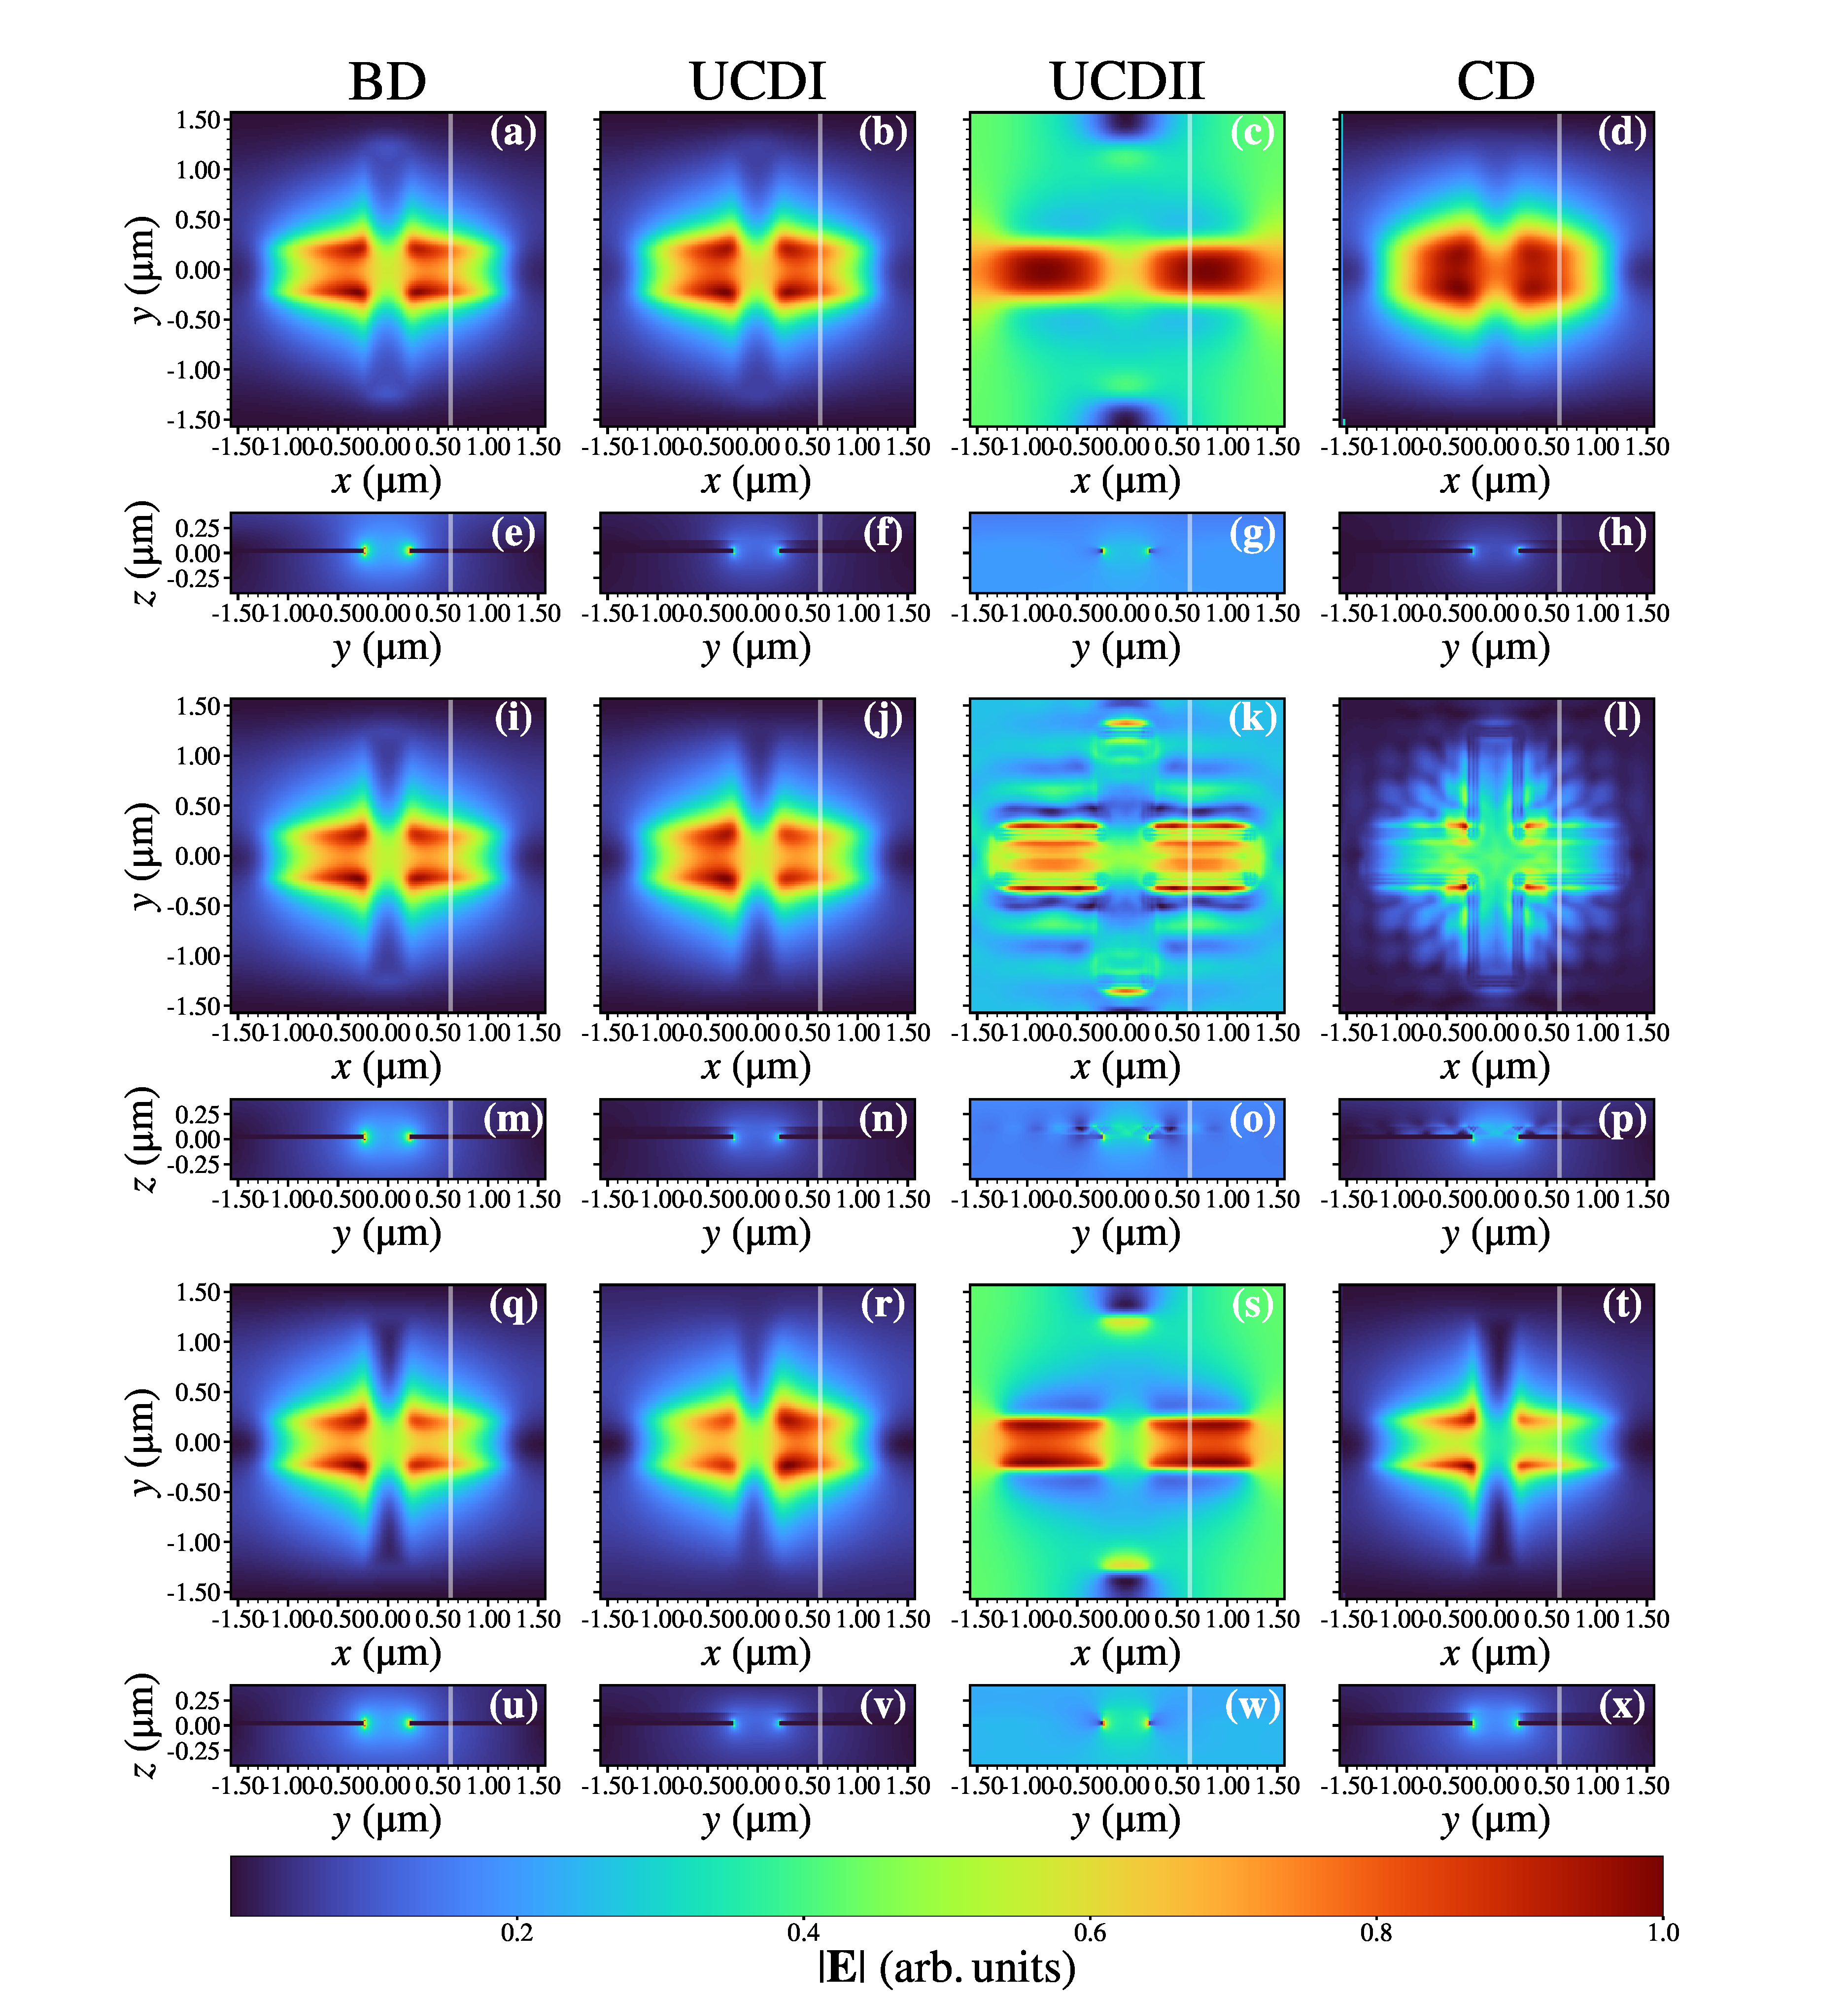
\includegraphics[width=0.9\textwidth]{Figures/Fig4.pdf}
				  \caption{ Background subtracted and normalized planar and cross-sectional colormaps of the field magnitude for the BD, UCDI, UCDII, and CD with $d_\mathrm{CC} = 3.14 \, \si{\um}$.  Panes (a) -- (h) were excited below the restrahlen band at $\nu = 1200 \, \mathrm{cm}^{-1}$. The white lines in the planar colormaps panes (a) -- (d) indicate the location of the cross-sectional colormaps in (e) -- (h). Panes (i) -- (p) were excited in the restrahlen band at $\nu = 1500 \, \mathrm{cm}^{-1}$. The white lines in the planar colormaps panes (i) -- (l) indicate the location of the cross-sectional colormaps in (m) -- (p). Panes (q) -- (x) were excited above the restrahlen band at $\nu = 1700 \, \mathrm{cm}^{-1}$. The white lines in the planar colormaps panes (q) -- (t) indicate the location of the cross-sectional colormaps in (u) -- (x). 
				  }
				  \label{fig:3.9}
				\end{figure}

		\section{Near-Field Line-Out Analysis}
		\label{sec:NFAII}
				For potential comparison to experiment, it is useful to analyze lineouts from field data of the type presented in Fig.~\ref{fig:3.9}. A series of lineouts for a CD with $d_\mathrm{CC} = 3.14 \, \si{\um}$ is shown in Fig.~\ref{fig:3.10} (a). The electric fields were frequency resolved in the range $\nu = 1490 - 1570 \, \mathrm{cm}^{-1}$. The position of the lineout is indicated by the white line in the insert of Fig.~\ref{fig:3.10} (b). Lineout data was only extracted outside of the cross region, \textit{i.e.,} where the hBN was supported by an Au layer. The peaks in $|\bm{E}|$ were determined using the peak fitting algorithm described above. A phonon-polariton wavelength was assigned by calculating the averages of the differences between successive peaks. These wavelengths were found to lie in the range $140 - 330 \, \si{\nm}$. These data were used to construct a dispersion curve as shown in Fig.~\ref{fig:3.10} (b). Additional insight can be obtained by examining the individual field components \cite{Klein:2014}, thus  a similar process was applied to the $E_y$ lineout data as shown in Fig.~\ref{fig:3.10} (c) and (d). As can be seen by comparing the plots in Fig.~\ref{fig:3.10} (b) and (d), the computed dispersion curves are similar although not identical, particularly at low values of $q$. 

				\begin{figure}[!htb]
				  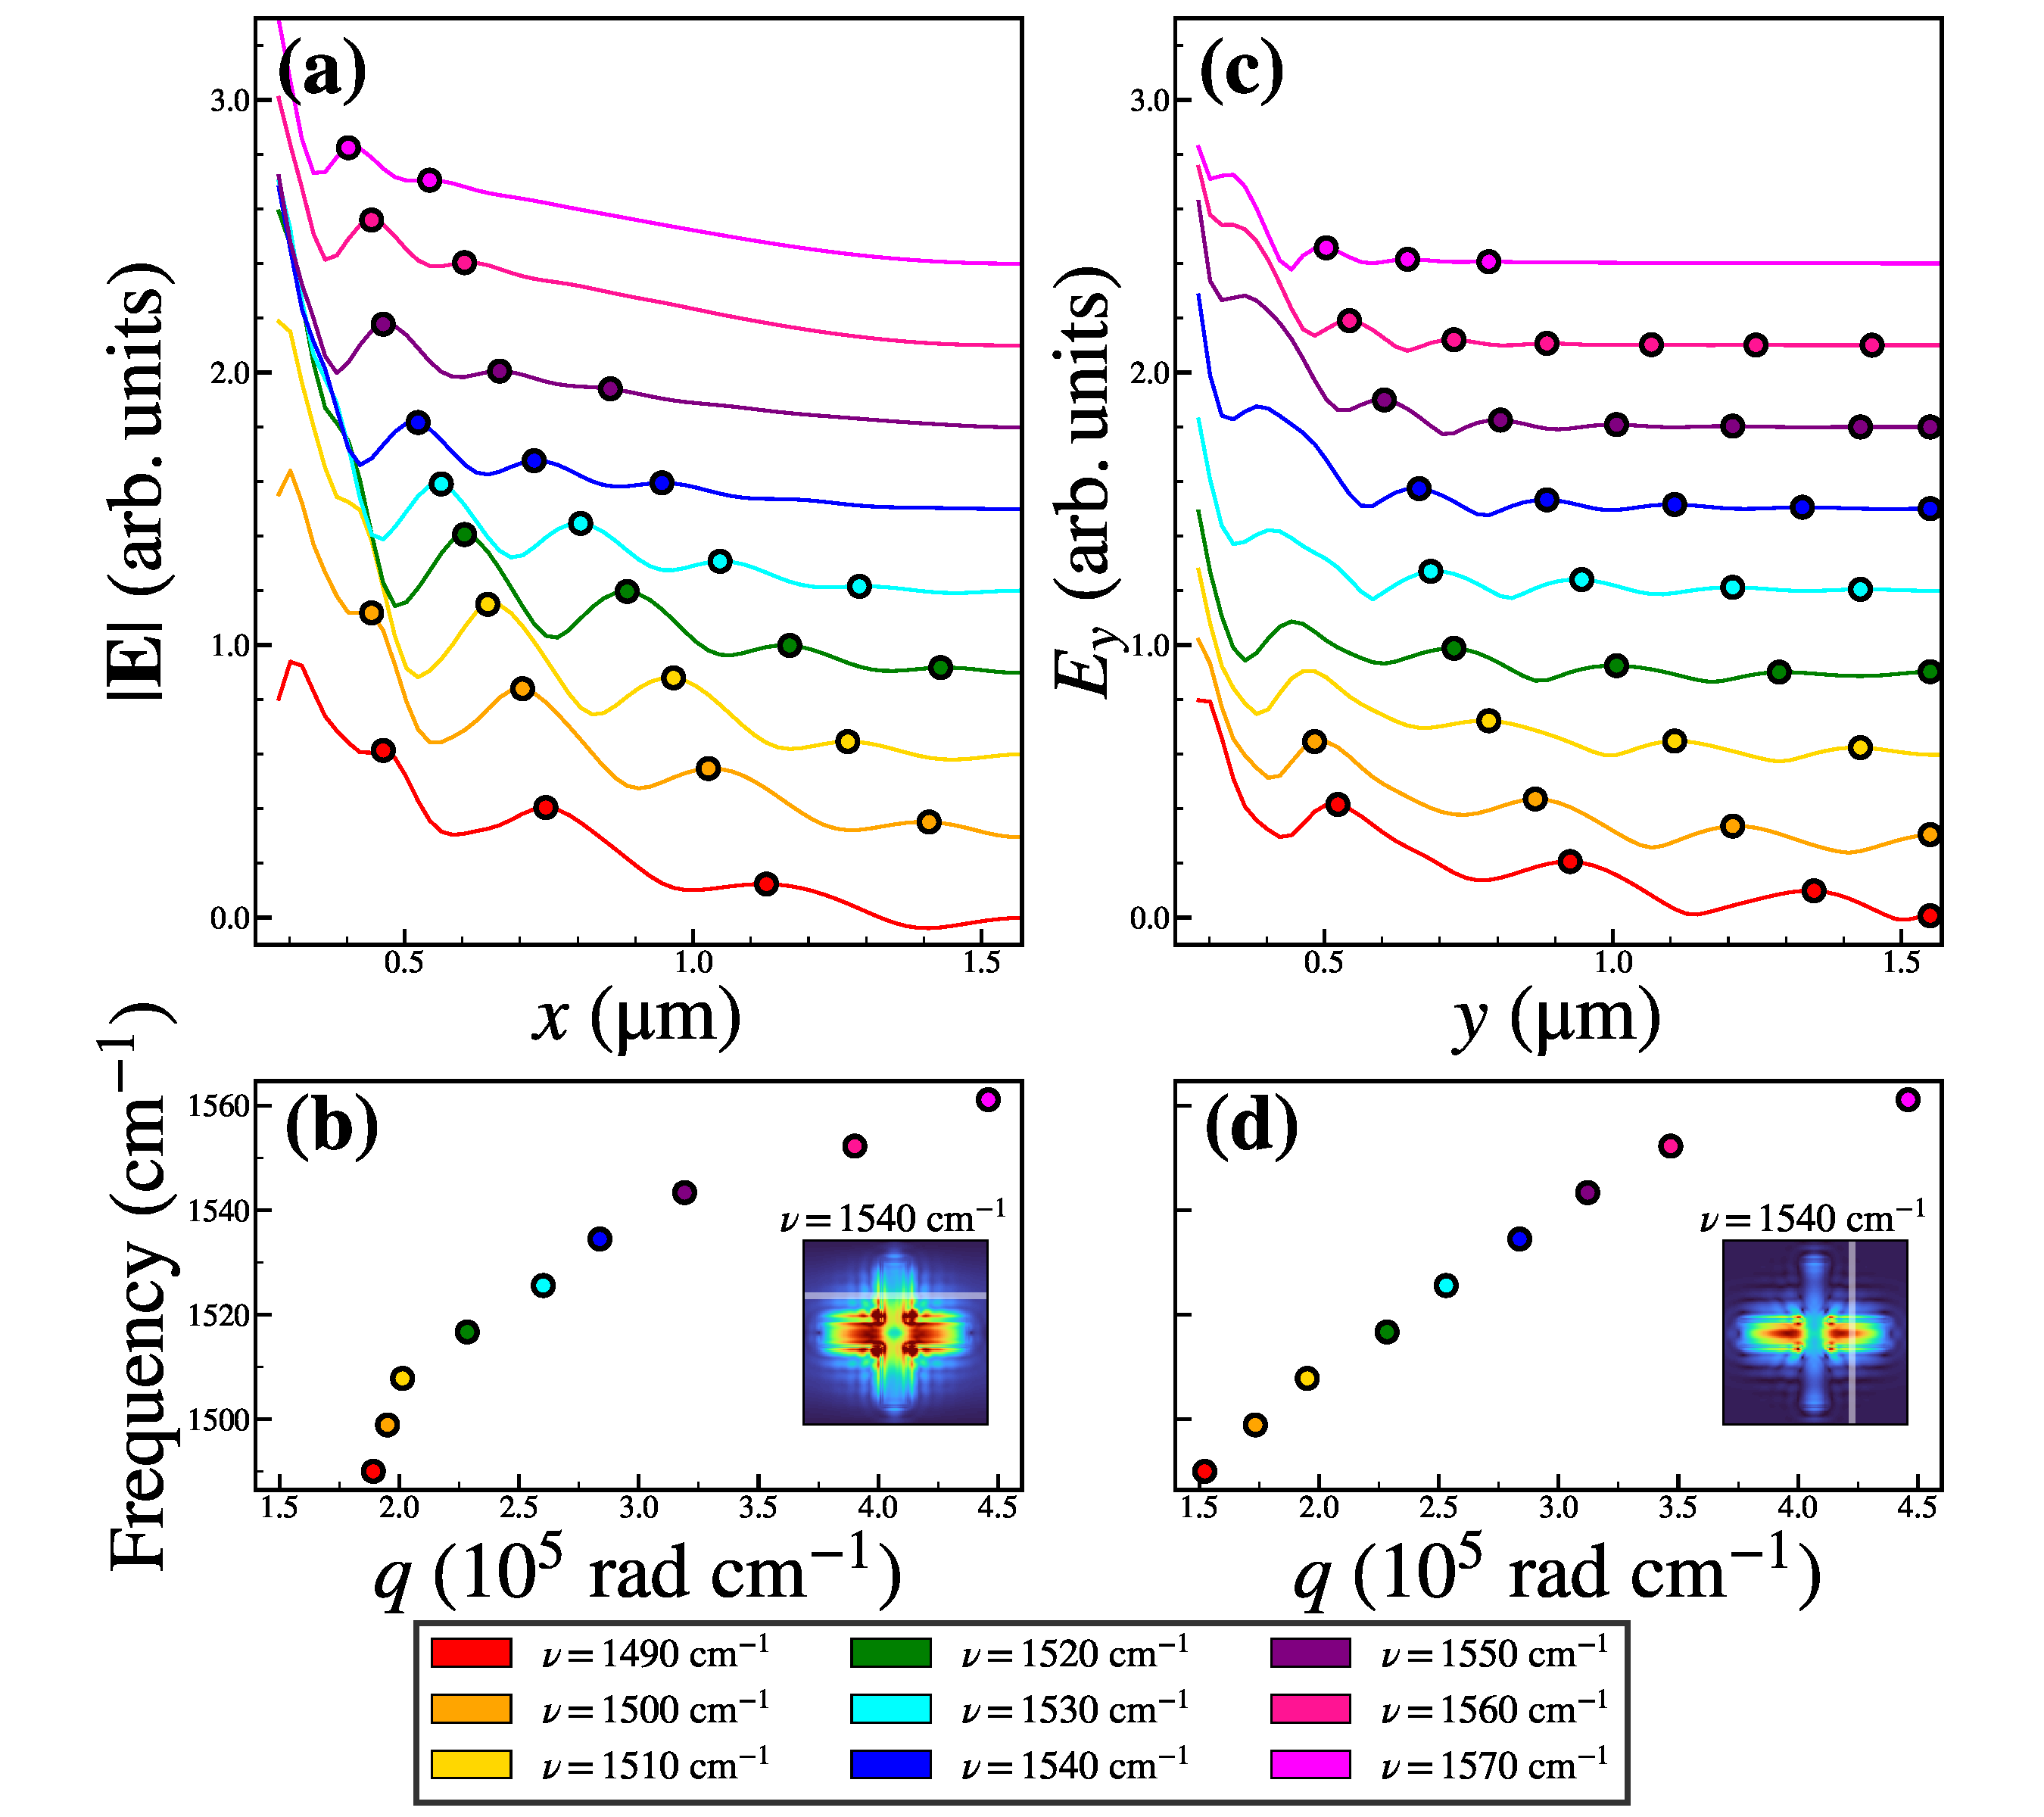
\includegraphics[width=0.9\textwidth]{Figures/Fig5.pdf} 
				  \caption{(a) Lineouts of the magnitude of the electric field for a range of excitation frequencies in the restrahlen band $\nu = 1490 - 1570\, \mathrm{cm}^{-1}$. The circular dots indicate peaks in the lineout. (b) Dispersion curve constructed from the peak data in pane (a). (c) Lineouts of the $y$-component of the electric field for a range of excitation frequencies in the restrahlen band $\nu = 1490 - 1570\, \mathrm{cm}^{-1}$. The circular dots indicate peaks in the lineout. (d) Dispersion curve constructed from the peak data in pane (c).The inserts in panes (b) and (d) show the position of the lineouts in panes (a) and (c).
				  }
				  \label{fig:3.10}
				\end{figure}	

		\section{Near-Field Line-Out Fourier Analysis}
		\label{sec:NFFA}

				Fig.~\ref{fig:3.11} (a) reproduces the far-field absorption spectrum from Fig.~\ref{fig:3.7} (c)  for convenient comparison with the near field data. Fig.~\ref{fig:3.11} (b) shows $E_y$ lineouts in the $y$-direction for frequencies in the range $\nu = 1000 - 1800\, \mathrm{cm}^{-1}$ at intervals of $1\, \mathrm{cm}^{-1}$. As can be seen from this figure, the region of highest field strength is in the vicinity of the inner Au|vacuum boundary within the cross (vacuum below the hBN layer), however features can be clearly resolved outside the cross (gold below the hBN layer). Broad features attributed to plasmons can be observed both below and above the restrahlen band; these features extend from inside the vacuum region into the gold region. Within the frequency range spanned by the restrahlen band, multiple branches can be observed in both the vacuum and Au regions. 

				\begin{figure*}[!htb]
				  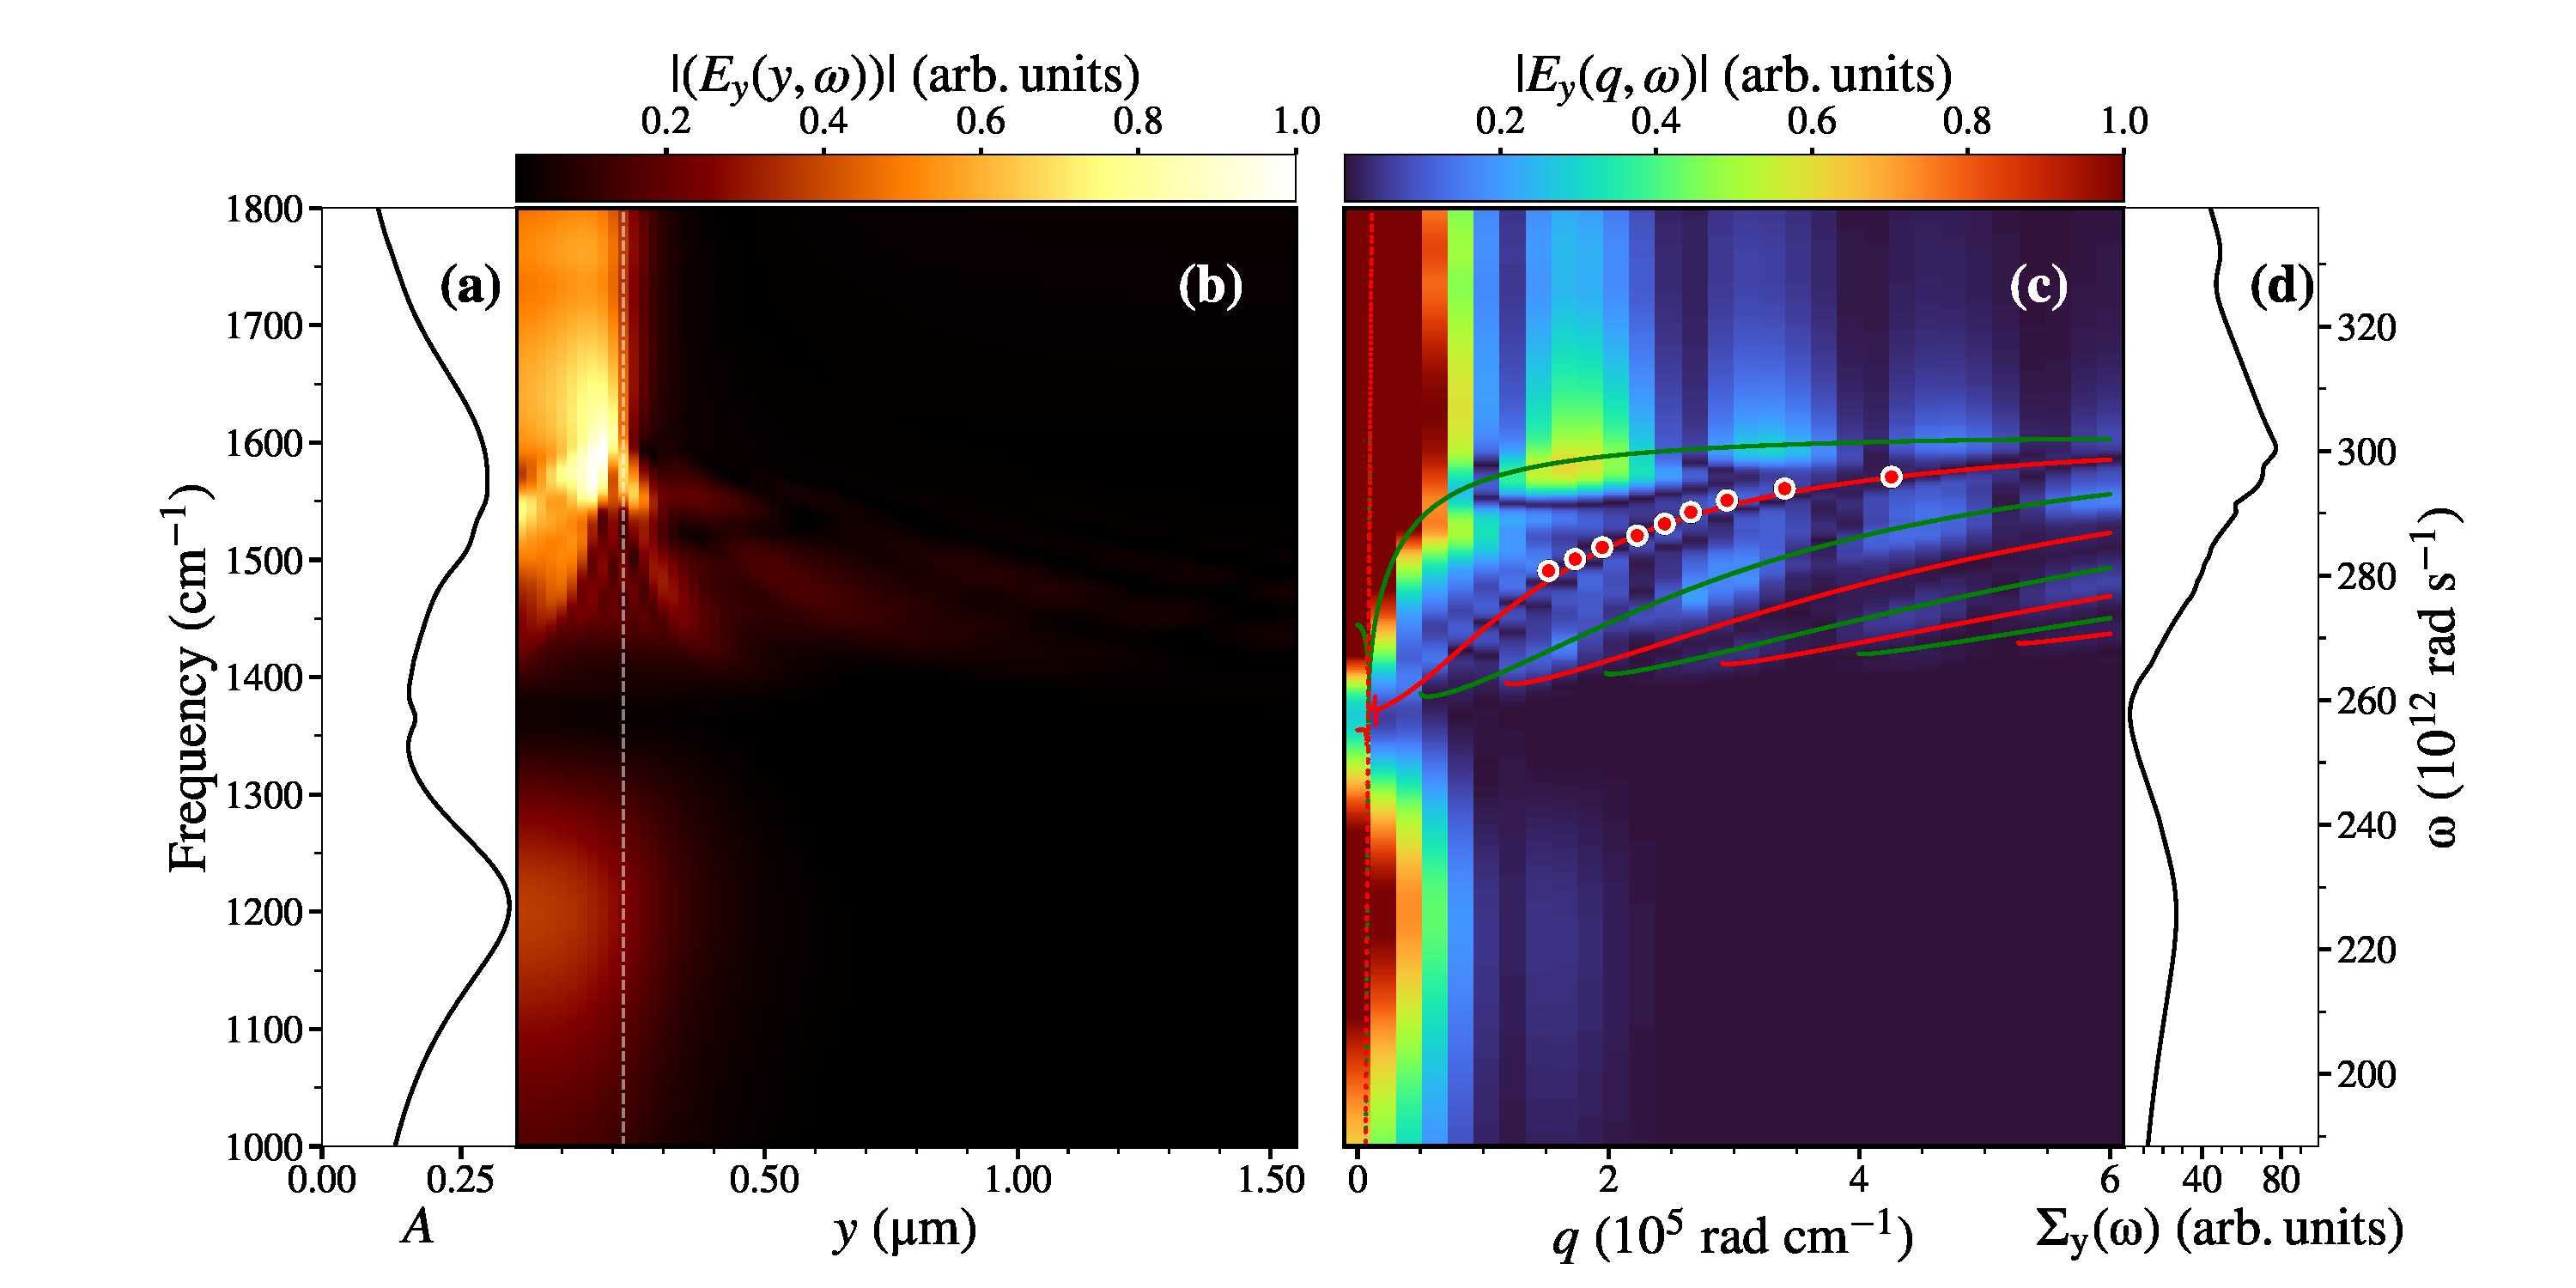
\includegraphics[width=0.9\textwidth]{Figures/Fig6.pdf}
				  \caption{(Color online) Phonon-polariton dispersion curves in the CD. (a) The far-field absorption spectrum. (b) $E_y$ lineouts (at the position of the white lines in Fig.~\ref{fig:3.9}) for frequencies in the range $\nu = 1490 - 1570\, \mathrm{cm}^{-1}$ with a spectral resolution of $1\, \mathrm{cm}^{-1}$. The spatial extent of the data displayed in this pane is from the center to the edge of the unit cell to avoid duplication. The white dotted line in this pane indicates the boundary between vacuum and Au. (c) The spatial Fourier transform of the (full spatial lineout) data presented in pane (b). The resulting plot of $|E_y(q,\omega)|$ enables the phonon-polariton dispersion curves to be visualized. The red and green theoretical dispersion curves are calculated as described in the text. The red dots are the dispersion curve data from Fig.~\ref{fig:3.10} (b). (d) The spectral content of the data in pane (c) obtained by integrating over $q$.
				  }
				  \label{fig:3.11}
				\end{figure*}
		
		\section{Theoretical Dispersion Curve Calculations}
		\label{sec:DCC}
		
				Fig.~\ref{fig:3.11} (c) shows the spatial Fourier transform of the (full spatial lineout) data described above. The resulting plot of $|E_y(q,\omega)|$ enables the phonon-polariton dispersion curves to be visualized. In order to aid the interpretation of the data in Fig.~\ref{fig:3.11} (c), theoretical phonon-polariton dispersion curves were calculated for a pair of three-layer thin-film structures: (i) Vacuum/hBN/Vacuum, and (ii) Vacuum/hBN/Au. The dispersion curves were calculated by finding the maxima of the imaginary part of the complex Fresnel reflection coefficient at real momenta as described in detail in the supplemental materials of the 2014 paper by Dai \textit{et al.} \cite{Dai:14}. The curves in green are for the  Vacuum/hBN/Vacuum structure, while the curves in red are for the Vacuum/hBN/Au structure. The dispersion curves calculated in this manner were in good agreement (in their region of overlapping validity, \textit{i.e.,} at high wavevector) with the dispersion curves calculated using the quasistatic approximation \cite{Dai:14, Kumar:15}, 
			
				\begin{align}
				  q(\omega)   = & -  \frac{\Psi}{d_\mathrm{hBN}} \left[  
				    \tan^{-1} \left\{ \frac{\varepsilon_0}{\varepsilon_{x,y}(\omega)\Psi} \right\} \right. \nonumber\\
				     & +  \left. \tan^{-1} \left\{ \frac{\varepsilon_\mathrm{s}}{\varepsilon_{x,y}(\omega)\Psi} \right\} + n\pi \right],
				  \label{DR}
				\end{align}
				\noindent where $\Psi = -i\sqrt{\varepsilon_z(\omega)/\varepsilon_{x,y}(\omega)}$ and $\varepsilon_{x,y,z}(\omega)$ are the components of the hBN dielectric tensor, $\bm{\varepsilon}_\mathrm{hBN}(\omega)$. $\varepsilon_\mathrm{s} = \varepsilon_0$, the permitivity of free space for the Vacuum/hBN/Vacuum structure and $\varepsilon_\mathrm{s} = \varepsilon_\mathrm{Au}(\omega)$ for the Vacuum/hBN/Au structure; $n$ is an integer and all other quantities are defined above. The advantage of Eq.~\ref{DR} is that it explicitly highlights that the phonon-polariton dispersion clearly has multiple branches, and that those branches are labelled by $n$.

				As can be seen in Fig.~\ref{fig:3.11} (c), the two upper green curves (dispersion curves for the Vacuum/hBN/Vacuum structure with $n$ = 0 and 1, respectively) overlap regions with large values of $|E_y(q,\omega)|$. It is notable that the value of $|E_y(q,\omega)|$ decreases strongly with increasing values of $n$. From Fig.~\ref{fig:3.11} (c) it is difficult to see direct evidence of the dispersion curves for the Vacuum/hBN/Au structure, since most of the field strength is concentrated in the vacuum region as noted above. However, the Vacuum/hBN/Au curves can be enhanced by using a windowing function to mask off the vacuum data in Fig.~\ref{fig:3.11} (b) before Fourier transforming that data. While this approach enables the $n=1$ dispersion curve for the Vacuum/hBN/Au structure to be directly visualized, it also introduces artifacts due to the windowing process; a more unambiguous approach is to plot the dispersion curve data shown in Fig.~\ref{fig:3.10} (d) on top of the data shown in Fig.~\ref{fig:3.11} (c). Good agreement is observed between these data (plotted as red circles) and the red $n=1$ dispersion curve for the Vacuum/hBN/Au structure.

				The spectral content of the data in Fig.~\ref{fig:3.11} (c) is obtained by integrating over $q$ to yield the quantity denoted $\Sigma_y(\omega)$, which is plotted in Fig.~\ref{fig:3.11} (d). The resulting spectrum, while exhibiting the broad features of the far-field spectrum, shows three notable differences. Firstly, this spectrum suppresses the residual peak at the hBN TO optical phonon frequency. Secondly, there is additional structure within the hBN restrahlen band, finally there is an additional peak centered at $\sim 1750\, \mathrm{cm}^{-1}$, the origin of which is not understood at this time. The near-field spectrum, $\Sigma_y(\omega)$, therefore emphasizes the slab phonon-polaritons over the bulk phonon-polaritons when compared to the far-field spectrum thus highlighting the importance of using near-field experimental techniques to investigate systems of this kind. 

		\section{Conclusions}
		\label{sec:Con}

			The excitations that occur in a hBN/nanopatterned Au device have been investigated using the Finite-Diffence Time-Doman (FDTD) method. In order to gain a more detailed understanding of the coupling between the phonon-polaritons in the hBN layer and the plasmon-polaritons in the nanopatterned Au layer, the far- and near-field properties of this coupled device (CD) were compared with the properties of three other uncoupled devices denoted BD (supports plasmon-polaritons only), UCDI (supports plasmon-polaritons only) and UCDII (supports phonon-polaritons only). An examination of the far-field absorption spectra of the above devices show that in the coupled device the absorptance peak, associated with the plasmon-polariton in UCDI, splits due to the interaction with the bulk phonon-polariton in hBN, while an examination of the absorption fine-structure provides evidence of slab phonon-polaritons in hBN.

			An investigation of the near-field electric field distributions enables the slab phonon-polaritons to be identified and categorized according to mode number per Eq.~\ref{DR} and supporting layer, \textit{i.e.,} vacuum or Au. A comparison of the field maps for the CD and UCDII show that the presence of the plasmon-polaritons in the CD increases the contrast in the spatial electric field variation indicating that the plasmon plays a key role in both coupling energy into the hBN phonon-polaritons and in launching phonon-polaritons into different directions within the hBN layer. It is hoped that the detailed simulations presented in this paper will be helpful in informing future experimental investigations of these interesting and technologically relevant systems.

\bibliography{hBNPaper.bib}
\end{document}		